\section{Experiments}




\fmc{TODO: Describir bien la intro a esta seccion, describiendo todas las subsecciones que contiene}

\textcolor{gray}{TODO: Explicación de los experimentos:
Introducción: qué contiene la sección
\begin{itemize}
    \item Explicación inicial de lo que queremos probar
    \item Cómo se va a probar:
    \begin{itemize}
        \item Evaluation metrics: diefficiency
        \item Different bank sizes
        \item Different streams
        \item Scaling for the NRT tests
        \item Measurement of all the checks, not only the alerts
    \end{itemize}
    \item Resultados
\end{itemize}
}

\fmc{Explicar la sección en base a este esqueleto}
\textcolor{blue}{Esqueleto:
\begin{itemize}
    \item Qué hago: Diseño / Experimentos / Evaluacion experimental planteada
    \item Dónde lo hago: Experimental Setting
    \item Cómo lo mido: Metrics
    \item Con qué lo hago: Datasets
\end{itemize}
}

In this section we detail the experimental evaluation done in order to show the performance of the \DPATM system. With these experiments we intend to show the suitability of the dynamic pipeline computational model as a real-time system capable of emitting results as they are computed, in a progressive way.\\

% Explicación breve de los dos principales tipos de experimentos que hemos hecho: RT and NRT-high load scenario
To evaluate the \DPATM as a real-time system, we conducted two kinds of experiments. On the one hand the analysis of the \DPATM on a high-load stress scenario (E1), where we study the behavior of the system in a worst case scenario, receiving a high loaded transaction stream. On the other hand, the evaluation of the \DPATM in scenarios reflecting more real-world possible conditions, with a more realistic transaction frequency (E2). In each of the cases we intend to show the performance of the system under different possible configurations in terms of the number of filters and available cores on the running machine.\\

% Metrics
To evaluate the behavior of the system in these scenarios, we decided to analyze not only classical real-time system metrics but also newly proposed metrics for assessing the system's continuous behavior in terms of the emitted results. The selection of the metrics for the system evaluation is described in \ref{exps:evaluation-metrics}. In \ref{exps:results-definition} we explain the possible considered definitions for a system result, which we will select depending on the experiment.\\

% Stream & bank sizes
The system will be tested for different possible bank sizes, with varying numbers of cards, ATMs, and stream sizes, simulating various time intervals of card-ATM interactions. The selection of the different possible bank and synthetic transaction stream sizes are given in \ref{exps:bank-stream-configs}. 

\fmc{Explicar que se empezaron a hacer los dos experimentos, pero que al hacer E2 se acabó viendo que realmente se estaba tendiendo a hacer el E1, y que por eso el principal experimento de referencia fue la prueba del sistema en un high-load scenario E1.}

Finally, we devote \ref{exps-input-reading} to discuss different considered methods to consume the stream of transactions, and the empirical comparisons from which we decided the method of stream consumption by the \DPATM in our experiments. Part of this discussion was already advanced in the description of the implementation of the \source \Sr stage in \ref{ContinuousQueryEngine}.

\subsection{Design of Experiments}
\fmc{Aquí explico los experimentos que pensamos para probar el sistema, E1 (evaluation in a high load scenario) y E2 (evaluation in a more real-case scenario)}

\subsubsection{E1: Evaluation in a High-Load Stress Scenario}
\fmc{TODO: Describir y poner resultados}
% Intro - Descripción general
In this section we evaluate the behavior of the \DPATM in worst-cases scenarios in terms of the frequency of the transactions of the input stream. This intends to prove the performance of the \DPATM in a stress scenario where the stream of transactions arriving to the system is at its maximum peak.\\

To evaluate the behavior of the system under these conditions, we decided to analyze not only classical real-time system metrics but also newly proposed metrics for assessing the system's continuous behavior. The selection of the metrics for the system evaluation is described in \ref{exps:evaluation-metrics}.\\

For the experiments perform The real-case scenario and the high loaded test scenario. In the first case, the interactions, although read by a file of artificial simulated interactions, are provided to the pipeline data stream in such a way that they simulate their actual arrival time to the system, with the corresponding time separation between them. In the second case, the interactions are provided just one after the other as fast as possible as they are read.\\

Continuous delivery of results in a high loaded scenario

\begin{itemize}
  \item Q2: Behavior of the different system variations on a high loaded transaction stream scenario.
  \item R2: Not real time simulation. Direct transaction stream input supply. Comparison of the continuous delivery of results of the different systems variations (diefficiency metrics).
\end{itemize}

\subsubsection{E2: Evaluation in a Real-World Stress Scenario}

\textcolor{blue}{
\subsection{Experimental setting} 
Hardware \& software
}
\fmc{Descripción de las versiones de nuestros programas (del Golang y del driver para la conexión go a Neo4j ya se describe en el apartado de la implementación del \DPATM.}
\fmc{Aquí más pues de dónde corrimos los experimentos, describir máquinas del cluster, etc}


\fmc{TODO: Hacer subapartado para dar bien los detalles de NEO4J en la VM y los detalles de como se hace la conexión a través de go, etc}
\paragraph*{Connection to GDB}

\textcolor{red}{TODO: Add this in the data model section under a new subsection?}

Some details / notes on how this is performed in golang.


So far:
\begin{itemize}
  \item \texttt{DriverWithContext} object: only 1, shared among all the threads. It allows connections and creation of sessions. These objects are immutable, thread-safe, and fairly expensive to create, so your application should only create one instance.
  \item \texttt{Sessions}: so far we create one session every time we do a \texttt{checkFraud()} operation.
  Session creation is a lightweight operation, so sessions can be created and destroyed without significant cost. Always close sessions when you are done with them. They are not thread safe: you can share the main DriverWithContext object
  across threads, but make sure each routine creates its own sessions.
  \item \texttt{context}: context variable is not unique, and we will create one different just before needing to call functions related with the connection module.
\end{itemize}


\textcolor{blue}{\textbf{CHANGED:} 1 session per filter.\\
However, note that many multiple parallel sessions may cause overhead to the database...}
... WE ARE GOING TO ASK THE ADMIN TO KNOW THIS... In the case this is a problem we will need
to think of the pool of connections.


Some notes on this:

\begin{itemize}
  \item \href{https://neo4j.com/docs/operations-manual/current/performance/bolt-thread-pool-configuration/}{Bolt thread pool configuration}: Since each active transaction will borrow a thread from the pool until the transaction is closed, it is basically the minimum and maximum active transaction at any given time that determine the values for pool configuration options: 
  \begin{itemize}
    \item \texttt{server.bolt.thread\_pool\_min\_size}: 5 by default.
    \item \texttt{server.bolt.thread\_pool\_max\_size}: 400 by default.
  \end{itemize}
\end{itemize}

\paragraph*{Neo4j Details - VM Neo4j}

Tenemos una VM con Neo4j con 4 cores y 20GB de RAM.

\textcolor{red}{TODO: Add details on the Neo4j gdb and in the specific details of the VM of the UPC cluster in which we have our Neo4j gdb instance. \\
$\rightarrow$ DETAILS ON directory: "TFM/NEO4J" \href{https://github.com/FCanfran/TFM-Neo4j}{TFM-NEO4J}}

\textcolor{lightgray}{
$\rightarrow$En su día nos instalasteis una MV con Neo4j. Hemos hecho algunas pruebas y de momento bien!
Sin embargo quería preguntaros acerca de cuál es el límite en el número de sesiones que pueden haber en paralelo  (vamos a tener varios procesos en paralelo y cada uno con una sesión abierta para hacer queries a la base de datos. Estas queries en principio son todas de lectura), para entonces dependiendo de esto, saber si esto nos limita a la hora de ajustar el número de procesos que vamos a tener en paralelo.
He encontrado alguna referencia aquí:
https://neo4j.com/docs/operations-manual/current/performance/bolt-thread-pool-configuration/
donde indican que el número máximo de transacciones activas en un momento dado por defecto está en 400... No sé si esto influye en el número de sesiones o no.\\ $\rightarrow$Pues he estado buscando información y no veo en ningún sitio donde el Neo4j limite el número de sesiones que pueda haber en paralelo. Sí que he encontrado que limita el número de transacciones paralelas a 1000 por defecto, pero nada más.\\ $\rightarrow$Lo mejor es que prepares algunos tests y lo pruebes empíricamente ;)
}

%%
%%
\subsection{Definition of a System Result}\label{exps:results-definition}

In principle, attending only to our system description, we consider a result - or equivalently, an answer of the \DPATM - to be synonymous with an alert, caused by a positive fraud check on a \filter stage.\\

For experimental purposes, we propose an alternative result definition, in which we consider a result to be equal to a fraud pattern check. That is, all the fraud pattern checks are considered as results on this definition, even if they are negative, i.e. when they do not derive in the creation of an alert. Considering all the fraud pattern checks as results is done only due to experimental purposes, in order to better analyze the continuous production of results by the \DPATM, reflecting all the fraud pattern checking that the system is undergoing. Note that, considering all the checks as results will derive in a communication overhead between the \filter \F stages and the \sink \Sk stage, where the results are gathered. However, on a production version of the \DPATM, we will utilize the original definition of a \DPATM system result - the alerts are the results - as there would be no interest in sending negative fraud pattern checks to \Sk. Only the positive fraud pattern checks - the alerts - are of interest in that case, therefore reducing at maximum the overhead in the communication channel between the $\mathsf{F}$'s and \Sk and the corresponding processing of results in \Sk.

\subsection{Metrics}\label{exps:evaluation-metrics}

The \DPATM is an intended to be real-time system for the detection of card-ATM anomalous interactions. As such its evaluation must capture classical metrics such as: mean response time of an answer/detection to be produced, throughput in terms of answers emitted per unit of time, the execution time to process a full stream. 
Additionally, we include other kinds of metrics to quantify and evaluate the efficiency of the system over a certain time period, the so-called \emph{diefficiency} metrics, introduced in \cite{exps-diefficiency}. Unlike the classical metrics, these metrics allow us to have a more complete picture on how the system is behaving during a given period of time, and not just a reduced final picture, by evaluating the progressive emission of results in that time period.

% Describo las métricas una a una en un listado
\begin{itemize}
    \item \textbf{Number of results: \texttt{checks} and \texttt{alerts} produced\\}
    Counters of the number of results that the system produces. Results can be either be counted only as alerts (positive fraud patterns), as fraud pattern checks, both positive (alerts) and negative, or as both at the same time, depending on the experiment. 
    \item \textbf{Response Time (\texttt{RT}) and Mean Response Time (\texttt{MRT})\\}
    \texttt{RT} captures the time it takes for the system to emit a result. It is the elapsed time from the moment an interaction arrives to the system until the result of its respective fraud pattern check is produced. A fine-grained description on how this metric was captured in the \DPATM system is included in \ref{exp-measuring-mrt}. The \texttt{MRT} is the average response time metric for all the results emitted by the system.
    \item \textbf{Execution Time (\texttt{ET})\\}
    It measures the total time (in seconds) that it takes for the system to consume/process a full input stream.
    \item \textbf{Throughput (\texttt{T})\\}
    It measures the number of results emitted per time unit. It is calculated as number of results divided by \texttt{ET}.
    \item \textbf{Interactions per second (\texttt{interactions/s})\\}
    It measures the number of interactions that the system is able to process per time unit. It is calculated as the total number of interactions that arrived to the system divided by \texttt{ET}.
    \item \textbf{Time to produce the First Tuple (\texttt{TFFT})\\}
    It is the time required by the system to produce/emit the first result.
    \item \textbf{\texttt{dief@t} and \texttt{dief@k} metrics\\}
    They measure the \emph{diefficiency} - the continuous efficiency of an engine over a certain time period in terms of the emission of results - and, as mentioned allow us to have a more complete picture on how the system is behaving during a given period of time, and not just a reduced final picture. \texttt{dief@t} measures the diefficiency of the engine while producing results in the first \emph{t} time units of execution time. The higher the value of the \texttt{dief@t} metric, the better the continuous behavior. \texttt{dief@k} metric measures the diefficiency of the engine while producing the first \emph{k} results, after the first result is produced. The lower the value of the \texttt{dief@k} metric, the better the continuous behavior.

    \item \textbf{Answer Trace\\}
    We provide a similar definition as the one in \cite{exps-diefficiency}. An answer tra
ce can be formally defined as a sequence of pairs $(t_1,r_1),...,(t_n,r_n)$, where $r_i$ is the $ith$ result produced by the engine and $t_i$ is the timestamp that indicates the point in time when $r_i$ is produced. We will record an answer trace for each of the experimental evaluations of the engine, since they provide valuable insights about the continuous efficiency - diefficiency.

\end{itemize}

To obtain the \texttt{dief@t} and \texttt{dief@k} metrics we used the \texttt{diefpy} tool \cite{exps-diefpy-tool}, which calculates them from the generated answer/result traces by our system. This tool provides us with other utilities for the visualization of the metrics on the obtained sets of results such as: the visualization of answer traces, the generation of radar plots to compare the \texttt{dief@t} with the other conventional/classical metrics, the generation of radar plots to compare the \texttt{dief@k} at different answer completeness percentages, among others.

We additionally extended/modified the tool for our specific needs. This was done in order to visualize other metrics, especially the \texttt{mrt}, but also others like the thoughtput \texttt{T}, \texttt{interactions/s} or the \texttt{TFFT}.

\fmc{TODO: explicar mejor la utilidad de medir dieft and diefk... resultados... answer trace si es muy bueno}

%%
\textcolor{blue}{
\subsection{Datasets}
Por qu\'e no tienes real datasets y tuviste que crear data sint\'etica y entoces:
Explica/justificas por qu\'e todos son sint\'eticos
}

\subsubsection{Synthetic Database Creation}
\textcolor{blue}{
\paragraph{Data generation}
Toda la explicación de c\'omo has generado los grafos sint\'eticos
xxxxxxx
}
As previously mentioned, given the confidential and private nature of bank data, it was not possible to find any real bank dataset. In this regard, we had to design and generate our own synthetic stable property graph bank database and stream of synthetic transactions. 

\ad{Hay que explicar porqué no servía y citar los artículos originales.}

In what follows we explain all the work related with the generation of the synthetic dataset that was used to build the stable graph databases and interaction data streams for the proof of concept of our system.

\subsubsection*{Reference Dataset: Wisabi Bank Dataset}

For the generation of our synthetic database and stream of transactions we considered to take as a standard data reference the \emph{Wisabi Bank Dataset}\footnote{\href{https://www.kaggle.com/datasets/obinnaiheanachor/wisabi-bank-dataset}{Wisabi bank dataset on kaggle}}, which is a fictional banking dataset publicly available in the Kaggle platform. We used it as a first base to do general customisable programs for the generation of synthetic bank datasets and streams of transactions.

The interest to use this bank dataset as a base was mainly because it is large enough and it also contained a card-ATM transactions dataset. Additionally, it provides good heterogeneity on the different kind of transactions: withdrawals, deposits, balance inquiries and transfers. 
The details of the \emph{Wisabi Bank Dataset} are summarized next.
 
\begin{itemize}
    \item 8819 customers.
    \item 50 different ATM locations.
    \item 2143838 card-ATM transactions records of the different customers during a full year (2022) on five different states of Nigeria (Federal Capital Territory, Lagos, Kano, Enugu and Rivers State).
\end{itemize}

The dataset consists on ten \emph{csv} tables each with different information which is summarized on Table~\ref{table:wisabi-summary}.

\begin{table}[H]
\centering
\begin{tabular}{|l|l|}
\hline
\textbf{Name of the Table}                                                                                               & \textbf{Description}                                              \\ \hline
enugu\_transactions                                                                                 & Transactions of Enugu state (350251 transactions)                     \\ \hline
fct\_transactions                                                                                   & Transactions of Federal Capital Territory state \\ & (159652 transactions) \\ \hline
kano\_transactions                                                                                  & Transactions of Kano state (458764 transactions)                      \\ \hline
lagos\_transactions                                                                                 & Transactions of Lagos state (755073 transactions)                     \\ \hline
rivers\_transactions                                                                                & Transactions of Rivers state (420098 transactions)                    \\ \hline
customers\_lookup                                                                                   & Data of the different cardholders (8819 cardholders)                 \\ \hline
atm\_location\_lookup                                                                               & Data of the different ATM locations (50 ATMs)                 \\ \hline
\begin{tabular}[c]{@{}l@{}}calendar\_lookup, hour\_lookup,\\ transaction\_type\_lookup\end{tabular} & Complementary data of the previous tables                \\ \hline
\end{tabular}
\caption{Wisabi Bank Dataset Tables Summary}
\label{table:wisabi-summary}
\end{table}

The main usage that we did of this dataset was the obtention of a geographical distribution of the ATM locations and the construction of a card/client \emph{behavior} based on the ATM-card transactions records provided.

In particular, as for the data model, we divide the creation of the synthetic dataset in two. On the one hand the creation of the stable bank dataset and on the other hand the creation of the synthetic and anomalous transactions dataset that will conform the data stream reaching our system.

\subsubsection*{Stable Bank Dataset Generation}

\paragraph{Bank dataset generator: \texttt{bankDataGenerator.py}\\\\}\label{bankDataGenerator}
To do the generation of a stable bank dataset we developed the Python program \texttt{bankDataGenerator.py}. 
To use it we only need to enter the bank properties' values, and the number of the bank ATMs (internal and external) \texttt{n} and Cards \texttt{m} to be generated. With this program we can generate the \emph{csv} files which define the bank dataset. A directory named \texttt{csv} will be created with the following files: 

\begin{itemize}
    \item \texttt{bank.csv}: bank entity.
    \item \texttt{atm.csv}: ATM entities.
    \item \texttt{card.csv}: card entities.
    \item \texttt{atm-bank-external.csv}: external ATM-bank relations.
    \item \texttt{atm-bank-internal.csv}: internal ATM-bank relations.
    \item \texttt{card-bank.csv}: card-bank relations.
\end{itemize}
To use it:
% How to use the bankDataGenerator

\begin{enumerate}
    \item Ensure to have a \texttt{wisabi} named directory with the \emph{csv} files downloaded from the \emph{Wisabi Bank Dataset} on Kaggle.\footnote{\href{https://www.kaggle.com/datasets/obinnaiheanachor/wisabi-bank-dataset}{Wisabi bank dataset on kaggle}}.
    \item Ensure to have the \texttt{behavior.csv} file or run \texttt{\$> python3 behavior.py} to create it.
    \item Run \texttt{\$> python3 bankDataGenerator.py} -- \textcolor{gray}{Run with Python3.6 version or higher} -- and introduce:
    \begin{enumerate}
        \item Bank properties' values.
        \item $n = |ATM|$, internal and external.
        \item $m = |Cards|$.
    \end{enumerate}
\end{enumerate}

In what follows we give the details on the generation of the instances of our static dataset entities.

\fmc{Esto ponerlo en otr sitio:}
\textcolor{gray}{
For simplicity and to do it in a more stepwise manner, we are going to first create all the CSV data tables for the nodes and for the relations in the corresponding format and then we will populate the Neo4j GDB with them.}

\paragraph{Bank entity: \texttt{bank.csv}\\\\}

Since a unique bank instance is considered, the values of the properties of the bank node are manually assigned, leaving them completely customisable (see an example on \ref{csv:bank}).

\begin{center}
\lstset{style=csvStyle}
\begin{lstlisting}[caption={Example of a bank.csv}, label={csv:bank}]
                    name,code,loc_latitude,loc_longitude
                    Niger Bank,NIGER,6.478685,3.368442
\end{lstlisting}
\end{center}

\paragraph{ATM entity: \texttt{atm.csv}\\\\}

We generate $\texttt{n = n\_internal + n\_external}$ ATMs (\texttt{n\_internal} ATMs owned by the bank and \texttt{n\_external} external ATMs not owned by the bank, but still accessible
for the bank customers to perform transactions). See an example in \ref{csv:atm}.

\begin{itemize}
    \item \textbf{ATM identifier}: \emph{ATM\_id}. It is assigned a different code depending on the ATM internal or external relation of the ATM with the bank: 
        \[
        \emph{ATM\_id} =
        \begin{cases} 
        bank\_code \text{-} i & 0 \leq i < \texttt{n\_internal } \text{if internal ATM}  \\
        EXT \text{-} i & 0 \leq i < \texttt{n\_external } \text{if external ATM}
        \end{cases}
        \]
    \item \textbf{Geographical properties}: \emph{city}, \emph{country}, \emph{loc\_latitude}         and \emph{loc\_longitude}. 
        They are assigned following the geographical distribution of the locations of the ATMs in the \emph{Wisabi Bank Dataset}. 
        On this dataset there are 50 ATMs locations distributed along Nigerian cities. 
        Note that for each of these ATMs locations, there can be more than one ATM.
        However, this is not taken into account and only one ATM per location is assumed for the 
        distribution. This distribution of the ATMs matches the relevance of the location in terms of its population, since the number of ATM locations is larger in the most populated 
        Nigerian cities (30\% of the ATM locations are in the city of Lagos, then the 20\% in Kano...).
        
        \fmc{Put plot of the ATMs geographical distribution?}
        \ad{Si, estaria bien, un ejemplo}
        
        With this, we assign each of the \texttt{n} ATMs \emph{city} and \emph{country} properties a random location/city from the \emph{Wisabi Bank Dataset}, and we then produce random geolocation coordinates inside the bounding box of the city location to set as the \emph{loc\_latitude} and \emph{loc\_longitude} properties of the ATM. \\
\end{itemize}

\begin{center}
\lstset{style=csvStyle}
\begin{lstlisting}[caption={Example of atm.csv}, label={csv:atm}]
                ATM_id,loc_latitude,loc_longitude,city,country
                NIGER-0,12.124651,8.543515,Kano,Nigeria
                NIGER-1,12.148756,8.481764,Kano,Nigeria
                EXT-0,8.941474,7.526291,Abuja,Nigeria
                EXT-1,4.816251,7.010188,Port Harcourt,Nigeria
\end{lstlisting}
\end{center}

\paragraph{Card entity: \texttt{card.csv}\\\\}

We generate a total of \texttt{m} cards that the bank manages. For each of them the assignment of the different properties is done as explained next. An example of a Card data item can be seen in \ref{csv:card}.

\begin{itemize}
\item \textbf{Card and client identifiers}:

\[
\begin{cases} 
number\_id = \text{c-}bank\_code\text{-}i \\
client\_id = i 
\end{cases}
0 \leq i < \texttt{m}
\]

\item \textbf{\emph{expiration} and \emph{CVC} properties}: they are not relevant, could be empty value properties indeed or a same toy value for all the cards. The same values are given for all the cards: $expiration = \text{2050-01-17}$, $CVC = 999$.

\item \textbf{Client's habitual address location (\emph{loc\_latitude}, \emph{loc\_longitude})}: two possible options were designed to define the client habitual residence address. In both 
cases they are random 
coordinates drawn from a bounding box of a location/city. The difference is on how the selection of the location/city is done:

  \begin{enumerate}
      \item \textbf{Wisabi customers selection}: take the city/location of the usual ATM of a random selected \emph{Wisabi} database customer. Note that in the \emph{Wisabi Bank Dataset} customers contain an identifier
      of their usual ATM, more in particular, the dataset is designed in such a way that customers
      only perform operations in the same ATM.
      With this approach, we maintain the geographical distribution of the \emph{Wisabi} customers.
      \item \textbf{Generated ATMs selection}: take the city/location of a random ATM of the \texttt{n} generated ATMs. This method is the one utilized so far.
  \end{enumerate}

\item \textbf{\emph{Behavior} properties}: these are properties of special interest both when performing the 
generation of the synthetic transactions of each of the cards and also for the detection of future possible fraud patterns. The defined \emph{behavior} properties are shown in Table \ref{table:behavior-properties}. They refer about metrics related with four different types of operations: withdrawal, deposit, balance inquiry and transaction. These operations will be the ones that, as in the base dataset, we will also consider that a customer can perform when we generate our synthetic transaction dataset.

\begin{table}[H]
    \centering
    \begin{tabular}{|l|l|}
        \hline
        \textbf{Behavior Property} & \textbf{Description} \\ 
        \hline
        $\mathsf{amount\_avg\_withdrawal}$ & Withdrawal amount mean\\ 
        \hline
        $\mathsf{amount\_std\_withdrawal}$ & Withdrawal amount standard deviation \\ 
        \hline
        $\mathsf{amount\_avg\_deposit}$ & Deposit amount mean \\ 
        \hline
        $\mathsf{amount\_std\_deposit}$ & Deposit amount standard deviation\\ 
        \hline
        $\mathsf{amount\_avg\_transfer}$ & Transfer amount mean \\ 
        \hline
        $\mathsf{amount\_std\_transfer}$ & Transfer amount standard deviation \\ 
        \hline
        $\mathsf{withdrawal\_day}$ & Average number of withdrawal operations per day \\ 
        \hline
        $\mathsf{deposit\_day}$ & Average number of deposit operations per day \\ 
        \hline
        $\mathsf{transfer\_day}$ & Average number of transfer operations per day \\ 
        \hline
        $\mathsf{inquiry\_day}$ & Average number of inquiry operations per day \\ 
        \hline
    \end{tabular}
    \caption{\emph{Behavior} properties}
    \label{table:behavior-properties}
\end{table}


The behavior properties' values are assigned to each of the cards by taking a random behavior \emph{row} from the \texttt{behavior.csv} file. This \texttt{behavior.csv} contains the gathered behavior metrics of each of the customers of the \emph{Wisabi Bank Dataset}. It was generated by using the Python program \texttt{behavior.py}. This program creates the behavior of each of the original customers of the \emph{Wisabi Bank Dataset} by doing a summary of all its transaction records on this base dataset.

Another possible way to assign the \emph{behavior} parameters could be the assignation
of the same behavior to all of the card instances. However, this method will provide less variability in
the generation of the synthetic transactions than the aforementioned method. 
Nevertheless, other taylored generation methods to generate different \emph{behavior} for 
each the cards could also be considered to similarly obtain this
variability.

\item \textbf{Card money amount extraction limit property}: \emph{extract\_limit}. We set it up by setting an upper bound based on the \emph{amount\_avg\_withdrawal} behavior metric of the card. Other possible ways could be chosen for assigning a value to this property.
    $$extract\_limit: amount\_avg\_withdrawal * 5$$
\end{itemize}

\begin{center}
\lstset{style=csvStyle}
\begin{lstlisting}[caption={Example of card.csv (Part 1)}, label={csv:card}]
    number_id,client_id,expiration,CVC,loc_latitude,loc_longitude,extract_limit
    c-NIGER-0,0,2050-01-17,999,8.92926,7.398833,121590.9
\end{lstlisting}
\end{center}

\begin{center}
\lstset{style=csvStyle}
\begin{lstlisting}[caption={Example of card.csv (Part 2)}]
        amount_avg_withdrawal,amount_std_withdrawal,withdrawal_day
        24318.18,28174.96,0.2411
\end{lstlisting}
\end{center}

\begin{center}
\lstset{style=csvStyle}
\begin{lstlisting}[caption={Example of card.csv (Part 3)}]
        amount_avg_deposit,amount_std_deposit,deposit_day,inquiry_day
        11500.0,5889.33,0.0548,0.0493
\end{lstlisting}
\end{center}

\begin{center}
\lstset{style=csvStyle}
\begin{lstlisting}[caption={Example of card.csv (Part 4)}]
        amount_avg_transfer,amount_std_transfer,transfer_day
        21448.28,20500.15,0.0795
\end{lstlisting}
\end{center}

\paragraph{ATM-Bank \texttt{interbank} relation: \texttt{atm-bank-external.csv}\\\\}

To represent the \texttt{interbank} relations between the bank and the external ATMs. Taking the unique ids of each of the related entities, the bank \emph{code} and the \emph{ATM\_id}. Example on \ref{csv:atm-bank-external}.

\begin{center}
\lstset{style=csvStyle}
\begin{lstlisting}[caption={Example of a atm-bank-external.csv}, label={csv:atm-bank-external}]
                                code,ATM_id
                                NIGER,EXT-0
                                NIGER,EXT-1
\end{lstlisting}
\end{center}

\paragraph{ATM-Bank \texttt{belongs\_to} relation:\texttt{atm-bank-internal.csv}\\\\}

To represent \texttt{belongs\_to} relations between the bank and the internal ATMs. Taking the unique ids of each of the related entities, the bank \emph{code} and the \emph{ATM\_id}. Example on \ref{csv:atm-bank-internal}.

\begin{center}
\lstset{style=csvStyle}
\begin{lstlisting}[caption={Example of a atm-bank-internal.csv}, label={csv:atm-bank-internal}]
                                code,ATM_id
                                NIGER,NIGER-0
                                NIGER,NIGER-1
                                NIGER,NIGER-2
\end{lstlisting}
\end{center}

\paragraph{Card-Bank \texttt{issued\_by} relation: \texttt{card-bank.csv}\\\\}

To represent the \texttt{issued\_by} relations between the bank and the card entities. Taking the unique ids of each of the related entities, the bank \emph{code} and the Card id: \emph{number\_id}. Example on \ref{csv:card-bank}.

\begin{center}
\lstset{style=csvStyle}
\begin{lstlisting}[caption={Example of a card-bank.csv}, label={csv:card-bank}]
                                code,number_id
                                NIGER,c-NIGER-0
                                NIGER,c-NIGER-1
                                NIGER,c-NIGER-2
\end{lstlisting}
\end{center}

\paragraph{\textcolor{blue}{Population of the Graph Database}\\}

% TODO: 
% 0. Description - Neo4j, what it is, why chosen...
% 1. Creation
% 2. Population

% Neo4j Desktop y version - instalación y detalles. Cómo conectarse...
% TODO: Explain how to install / connect... all the details that are in the neo4.md file
\textcolor{red}{$\rightarrow$ TODO: 0. Describe on how to set up the database}
\textcolor{red}{$\rightarrow$ TODO: Explanation of the versions of both Neo4j instances used - local and UPC VM cluster.}\\

Prior to the population of the Neo4j graph database, a Neo4j graph database instance needs to be
created. This was done both locally and in a \textcolor{red}{Virtual Machine of the UPC cluster}.

Version: Neo4j 5.21.0 Community edition. 
\begin{itemize}
    \item Accessing it: by default it runs on localhost port 7474: \texttt{http://localhost:7474}.
    Start the neo4j service locally by: \texttt{sudo systemctl start neo4j}\\
    It can be also be accessed by the internal utility \texttt{cypher-shell}. Username: \texttt{neo4j} and password: \texttt{bisaurin}.
\end{itemize}

\subsubsection*{Neo4j graph database population - CSV to PG}
\begin{comment}
    - Creación de la GDB - de CSV a Neo4j PG: 
    - Poner primero los comandos cypher por separado, con las constraints de uniqueness
    y luego lo de poblar. Luego ya referir a que todo ello se tiene en un único script que 
    permite la ejecución directa (en lugar de paso a paso) en golang.
    - Incluir detalles específicos de cada CSV...
\end{comment}

Once we created the Neo4j graph database instance and all the CSV data files representing all the nodes and relations, we populate the Property Graph instance in Neo4j. Before performing the population of the GDB, we create uniqueness constraints on the properties of the nodes that we use as our \emph{de facto} IDs for the ATM and Card IDs: \texttt{ATM\_id} and \texttt{number\_id}, respectively. The reason to do this is to avoid having duplicated nodes of these types with the same ID in the database. Therefore, as an example, when adding a new ATM node that has the same \texttt{ATM\_id} as another ATM already existing in the database, we are aware of this and we do not let this insertion to happen. ID uniqueness constraints are created with the following cypher directives:

\begin{center}
\lstset{style=cypherStyle}
\begin{lstlisting}[caption={Uniqueness ID constraints}]
            CREATE CONSTRAINT ATM_id IF NOT EXISTS
            FOR (a:ATM) REQUIRE a.ATM_id IS UNIQUE
    
            CREATE CONSTRAINT number_id IF NOT EXISTS
            FOR (c:Card) REQUIRE c.number_id IS UNIQUE
    
            CREATE CONSTRAINT code IF NOT EXISTS
            FOR (b:Bank) REQUIRE b.code IS UNIQUE
\end{lstlisting}
\end{center}

Once we created the Neo4j graph database instance and all the CSV data files representing all the nodes and relations, we populate the Property Graph instance in Neo4j. For this, we propose two different methods. The first does it by directly importing the CSV files using the Cypher's \texttt{LOAD CSV} command, while the second method does it by parsing the CSV data and running the creation of the nodes and relationships using Cypher. Both methods can be found and employed using the \texttt{populatemodule} golang module.
In this module we can find the two subdirectories where each of the methods can be run. In detail, the module tree structure is depicted in Figure \ref{fig:populatemodule}. On it, the \texttt{cmd} subdirectory contains the scripts to run each of the populating methods: the first method script on \texttt{csvimport} and the second on the \texttt{cypherimport}, while the \texttt{internal} subdirectory is a library of the files with the specific functions used by these methods.

\begin{figure}[h]
\centering
\begin{forest}
  for tree={
      font=\ttfamily,              % Typewriter font for file names
      grow'=0,                      % Tree direction (left-to-right)
      child anchor=west,            % Children alignment
      parent anchor=east,           % Parent alignment
      anchor=west,                  % Tree alignment
      calign=first,                 % Aligns with the first child
      edge path={
          \noexpand\path [draw, thick, \forestoption{edge}] (!u.parent anchor) -- +(-1pt,0) |- (.child anchor)\forestoption{edge label};
      },
      inner sep=4pt,
      l=10pt,                       % Level distance
      s sep=5pt                     % Sibling distance
  }
  [populatemodule
      [cmd
        [csvimport
            [main.go]
            [.env]
        ]
        [cypherimport
            [main.go]
            [.env]
        ]
      ]
      [internal
          [common
              [common.go]
          ]
          [populate
              [populate.go]
          ]
      ]
  ]
\end{forest}
\caption{\texttt{populatemodule} file structure}
\label{fig:populatemodule}
\end{figure}

% How to run it - .env file
% Description of each of the methods


Prior to run any of these methods we need to first set up correctly the \texttt{.env} file located inside the desired method directory, where we have to define the corresponding Neo4j URI, username and password to access the Neo4j graph database instance.

\begin{itemize}
\item{\textbf{Method 1: Cypher's \texttt{LOAD CSV}}\\}
The Cypher's \texttt{LOAD CSV} clause allows to load CSV into Neo4j, creating the nodes and relations expressed on the CSV files (see \href{https://neo4j.com/docs/cypher-manual/5/clauses/load-csv/}{\textit{load-csv cypher manual}}). 
To use it simply follow these steps:
\begin{enumerate}
    \item Place all the CSVs (\texttt{atm.csv}, \texttt{bank.csv}, \texttt{card.csv}, \texttt{atm-bank-internal.csv}, \texttt{atm-bank-external.csv} 
    and \texttt{card-bank.csv}) under the \texttt{/var/lib/neo4j/import} directory
    of the machine containing the Neo4j graph database instance.
    \item Run \texttt{\$> go run populatemodule/cmd/csvimport/main.go}
\end{enumerate}

\paragraph{Process description:}

Then the different CSV files containing all the data tables of our data set, were loaded into the GDB with the following cypher directives.

% TODO: Esto es en mi local. Se recomienda por razones de seguridad... Sin embargo se puede configurar para que no sea
% así. - En el cluster veremos. De momento no pongo nada de esto!
% First, the CSV files were needed to be placed under the \texttt{/var/lib/neo4j/import} directory.

\paragraph{ATM (atm.csv)}

\begin{center}
\lstset{style=cypherStyle}
\begin{lstlisting}[caption={atm.csv}]
    LOAD CSV WITH HEADERS FROM 'file:///csv/atm.csv' AS row
    MERGE (a:ATM {
        ATM_id: row.ATM_id,
        loc_latitude: toFloat(row.loc_latitude),
        loc_longitude: toFloat(row.loc_longitude),
        city: row.city,
        country: row.country
    });
\end{lstlisting}
\end{center}

Some remarks:
\begin{itemize}
    \item \texttt{ATM} is the node label, the rest are the properties of this kind of node.
    \item Latitude and longitude are stored as float values; note that they could also be stored
    as cypher \textit{Point} data type. However for the moment it is left like this. In the future
    it could be converted when querying or directly be set as cypher point data type as property.
\end{itemize}

\paragraph{Bank (bank.csv)}

\begin{center}
\lstset{style=cypherStyle}
\begin{lstlisting}[caption={bank.csv}]
    LOAD CSV WITH HEADERS FROM 'file:///csv/bank.csv' AS row
    MERGE (b:Bank {
        name: row.name, 
        code: row.code, 
        loc_latitude: toFloat(row.loc_latitude), 
        loc_longitude: toFloat(row.loc_longitude)
    });
\end{lstlisting}
\end{center}

Note that the \texttt{code} is stored as a string and not as an integer, since to make it more clear it 
was already generated as a string code name.

\paragraph{ATM-Bank relationships (atm-bank-internal.csv and atm-bank-external.csv)}

\begin{center}
\lstset{style=cypherStyle}
\begin{lstlisting}[caption={atm-bank-internal.csv}]
    LOAD CSV WITH HEADERS FROM 'file:///csv/atm-bank-internal.csv' AS row
    MATCH (a:ATM {ATM_id: row.ATM_id})
    MATCH (b:Bank {code: row.code})
    MERGE (a)-[r:BELONGS_TO]->(b);
\end{lstlisting}
\end{center}

\begin{center}
\lstset{style=cypherStyle}
\begin{lstlisting}[caption={atm-bank-external.csv}]
    LOAD CSV WITH HEADERS FROM 'file:///csv/atm-bank-external.csv' AS row
    MATCH (a:ATM {ATM_id: row.ATM_id})
    MATCH (b:Bank {code: row.code})
    MERGE (a)-[r:INTERBANK]->(b);
\end{lstlisting}
\end{center}

\paragraph{Card (card.csv)}

\begin{center}
\lstset{style=cypherStyle}
\begin{lstlisting}[caption={card.csv}]
    LOAD CSV WITH HEADERS FROM 'file:///csv/card.csv' AS row
	MERGE (c:Card {
		number_id: row.number_id, 
		client_id: row.client_id, 
		expiration: date(row.expiration), 
		CVC: toInteger(row.CVC), 
		extract_limit: toFloat(row.extract_limit), 
		loc_latitude: toFloat(row.loc_latitude), 
		loc_longitude: toFloat(row.loc_longitude),
		amount_avg_withdrawal: toFloat(row.amount_avg_withdrawal),
		amount_std_withdrawal: toFloat(row.amount_std_withdrawal),
		withdrawal_day: toFloat(row.withdrawal_day),
		amount_avg_deposit: toFloat(row.amount_avg_deposit),
		amount_std_deposit: toFloat(row.amount_std_deposit),
		deposit_day: toFloat(row.deposit_day),
		inquiry_day: toFloat(row.inquiry_day),
		amount_avg_transfer: toFloat(row.amount_avg_transfer),
		amount_std_transfer: toFloat(row.amount_std_transfer),
		transfer_day: toFloat(row.transfer_day)
		});
\end{lstlisting}
\end{center}

Notes:
\begin{itemize}
    \item We include the fields that were generated to define the behavior of the card. They are also used for the generation of the transactions.
    \item \texttt{expiration}: set as \textit{date} data type.
\end{itemize}

\paragraph{Card-Bank relationships (card-bank.csv)}

\begin{center}
\lstset{style=cypherStyle}
\begin{lstlisting}[caption={card-bank.csv}]
    LOAD CSV WITH HEADERS FROM 'file:///csv/card-bank.csv' AS row
    MATCH (c:Card {number_id: row.number_id})
    MATCH (b:Bank {code: row.code})
    MERGE (c)-[r:ISSUED_BY]->(b);
\end{lstlisting}
\end{center}

%\subsubsection*{Dataset extensions}

\begin{comment}
- Interesting reference for coordinates and distances in cypher - https://lyonwj.com/blog/spatial-cypher-cheat-sheet 
- Transactions dataset Generation  - a transaction dataset simulator → useful with the description of fraud scenarios, that can be generated among the transactions dataset, also with customers and terminals info generation (similar to ATMs concept) 
\end{comment}

\item {\textbf{Method 2: Creation of Cypher queries\\}}

\textcolor{red}{$\rightarrow$ TODO: Describe the other population method}

\textcolor{red}{$\rightarrow$ TODO: Describe the details of the VM of the UPC cluster where the gdb is hosted -- in TFM-Neo4j/size-estimaºtion, the gmail and other files...}

\end{itemize}


\textcolor{blue}{
\subsubsection{Considered datasets}
Haces una tabla con las caracteristicas de cada dataset (nvertices, nedges, density, par\'ametros  que te parezcan importantes (\smallG y \mediumG)
}

Bank Sizes:
\begin{itemize}
    \item \smallG: $|Card| = 2000$, $|ATM| = 50$
    \item \mediumG: $|Card| = 500000$,  $|ATM| = 1000$
\end{itemize}
%%
%%
% Apartado tamaños de banco y streams
\subsection{Stream Configurations}\label{exps:bank-stream-configs}
\fmc{Aqui describo como elijo el tamaño, el ratio de fraude y como genero / programa creado para generar los synthetic data streams}

Testing a bank system application like the \DPATM system implies deciding on different representative bank sizes and different stream sizes on which to perform the evaluation of the system. Regarding the stream of transactions the proportion of regular vs anomalous transactions also needs to be decided.\\

We did a brief investigation of some related works, regarding the experimental stream sizes as well as the ratio on the anomalous fraud transactions they utilize. On \cite{exps-atmfrauddetectionstreamdata} the authors propose an ATM fraud detection system based on ML models where they experiment with a transaction stream of a size close to $10^{6}$ consisting of a ratio of 0.88 regular operations to 0.12 fraudulent operations. In \cite{exps-costsensitivepayment} they propose a ML algorithm based on dynamic random forests and k-nearest neighbors, and they test it with a real bank transaction stream of $\sim5 \times 10^{4}$, representing the card activity of 415 different cards, with a fraudulent transaction ratio of 0.07. Finally in \cite{exps-featureengineering} they evaluate the impact of their proposed feature extraction techniques for credit card fraud detection on different ML and data mining state-of-the-art models. For their experiments they used a real European transaction dataset containing $\sim120 \times 10^{6}$ transactions representing a 18 months time interval, in which only $\sim40000$, that is a $0.025\%$, are fraudulent. They also consider a smaller subset of $\sim 2 \times 10^{5}$ transactions with a fraud ratio of $1.5\%$.

\fmc{TODO: Poner mejor}
Based on these references we constructed different streams with sizes and fraud ratio similar to the ones mentioned, using our generator of synthetic transactions, generated from different bank databases.
The variation on the size of the simulated stream of transaction on which to test our system is not the unique we do, we also variate the bank database size in terms of the number of cards and ATMs it contains. This variation, apart from having an influence on the volume of generated transactions on a time interval when using our synthetic transaction stream generator, it is expected to have an influence on the performance of the system due to the expected added overhead when querying the Neo4j stable graph database. In our experiments we propose two bank database sizes; one small bank database with 2000 cards and 50 ATMs, and one large bank database with 500000 cards and 1000 ATMs. 

\fmc{Poner referencias a bancos reales de tamaños similares?}


When generating the streams, in order to obtain the desired stream sizes, we needed to consider that our transaction generator takes as base the behavior of the clients of the 
Wisabi Bank Database, where each client typically produces at most $\sim 1$ transaction per day. (\textcolor{red}{TO CHECK to give the exact number}). This means that for each of the bank sizes being tested, in order to achieve the desired stream size, we need to decrease/increase the size of the time interval to be simulated.


\fmc{TODO: Sacar métricas exactas de cuál es el numero medio de ops por cliente de wisabi para poder decir cuál es el número de tx por dia approx que generamos con nuestro generador para poder relacionarlo}

\fmc{ Pongo esto?:Note that, for simplicity, we are assuming the number of bank branches as the number of ATMs and the number of clients as the number of cards.}

\begin{comment}

Sobre el número de cards y ATMs algunos bancos pequeños en España como la caja rural de Aragón tienen 14000 clientes y en torno a 200 sucursales (que podemos asumir como el número de ATMs, aunque sería algo más al tener más de 1 ATM por sucursal lo más seguro). Otros bancos pequeños (tipo cajas rurales) también suelen tener en torno a 100-200 sucursales y  algunos incluso 10^5 clientes.

En cuanto al número de transacciones, he estado mirando y algunos artículos juegan con un set de transacciones de en torno a 10^6 o 10⁵. Considerando que nuestro generador de transacciones como mucho crea una transaccion por card por día (basado en los datos del wisabi). Podríamos generar 1 mes de transacciones para 15000 cards y 200 ATMs, que podría dar  como mucho un stream de unas 450000 transacciones. 

\end{comment}

\fmc{Esto ponerlo solo aqui? Quitar contenido de la parte del source en la descripción de su impl. y hacer referencia solo a esto?}

\subsubsection*{Transaction Stream Generation}

% Details on the process. How the generation is done.
% How to run.
% Files generated. Show example of the csv.

The transaction set constitutes the simulated input data stream continuously arriving to the system. Each transaction represents the operation done by a client's card on a ATM of the bank network with the form of an \emph{interaction} edge/relation of the volatile subgraph (see \ref{section:volatile-pg}) matching one Card with one ATM of the bank database. In what follows we explain the generation of the transaction stream that we employed in order to test our system. Note that, in any case, this is only a possible proposal done with the intention of reproduce a close-to-reality bank transaction stream.

\textcolor{red}{\rule{\linewidth}{0.5mm}}
\fmc{TODO: Explain why we did this division open/close of the interaction...Dónde poner esta explicación?. Es importante, pues es una de las claves que pueden diferenciar/hacer a nuestro sistema diferente, capaz de hacer una detección de fraude en tiempo real}

\begin{figure}[h]
  \centering
  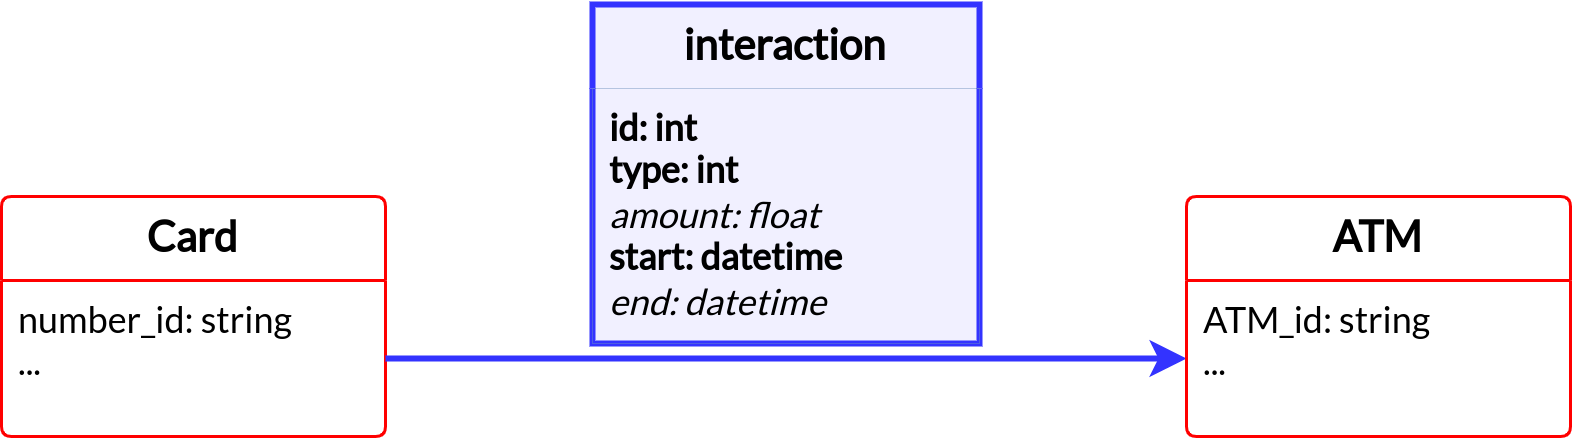
\includegraphics[scale = 0.8]{images/1-DataModel/2-edges-tx-tfm.png}
  \caption{\emph{Opening} interaction edge}
  \label{img:opening-edge}
\end{figure}

\fmc{Esto ponerlo en la definicion de interaction dentro de la definicion de volatile property graph del punto anterior}
It is important to remark that, \textcolor{gray}{as in our definition of the input data stream of the $DP_{CQE}$}, we generate two edges per transaction/\texttt{interaction} relation -- the \emph{opening} and the \emph{closing} edges -- which both will constitute a single \texttt{interaction} relation. The \emph{opening} edge (Figure \ref{img:opening-edge}) will be the indicator of the beginning of a new interaction between the matched Card and ATM, it contains the values of the properties related with the starting time \emph{start}, the interaction \emph{type} as well as the \texttt{id}. The \emph{closing} edge (Figure \ref{img:closing-edge}) will indicate the end of the interaction, completing the values of the rest of the properties of the interaction: \emph{end} and \emph{amount}.

\begin{figure}[h]
  \centering
  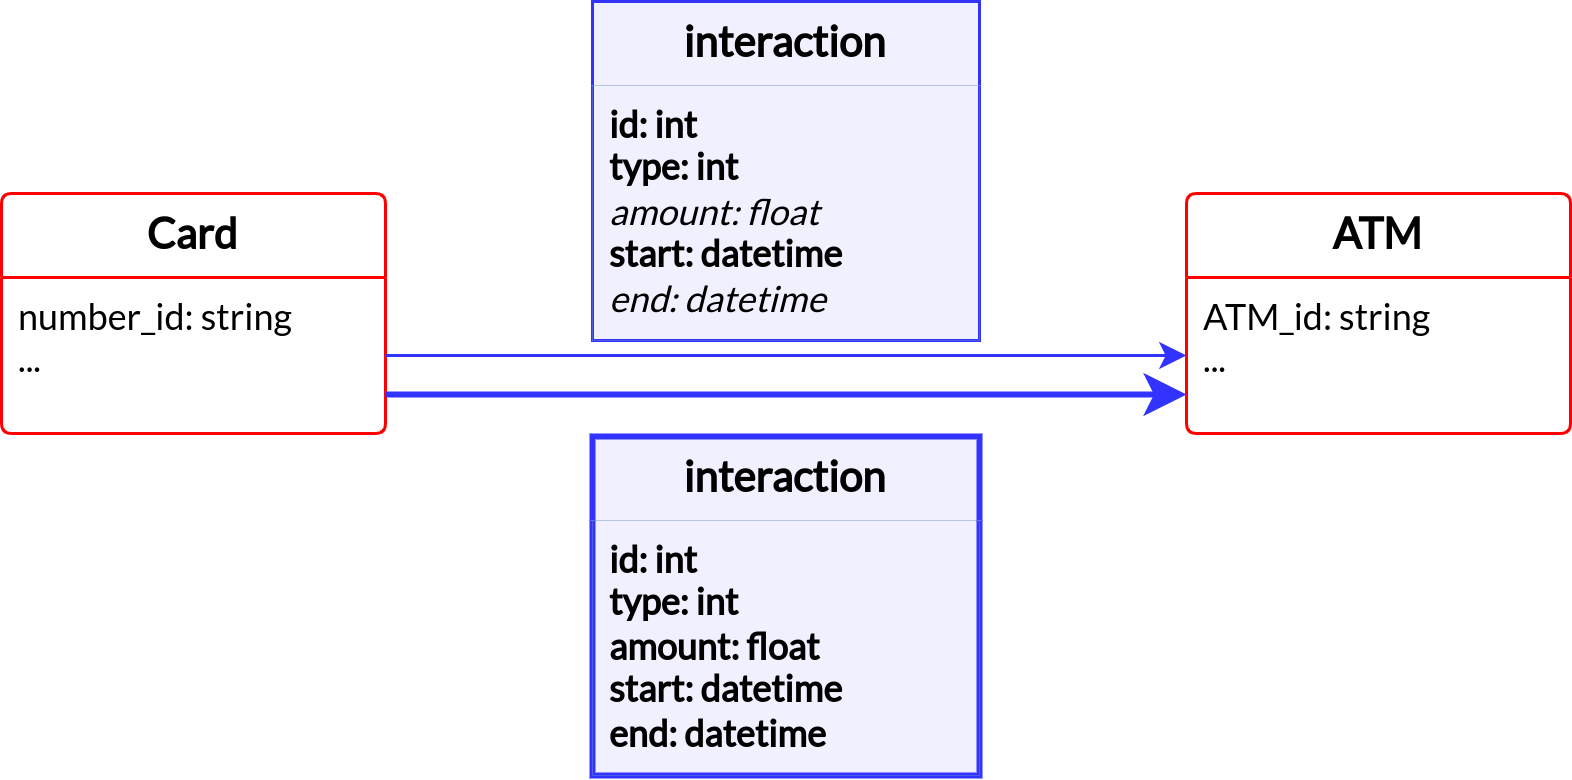
\includegraphics[scale = 0.8]{images/1-DataModel/2-edges-tx-tfm-1.png}
  \caption{\emph{Closing} interaction edge}
  \label{img:closing-edge}
\end{figure}

\textcolor{gray}{With this division of the interaction relation in two edges we are simulating that on each transaction, our system receives an initial message when the interaction starts and a final message once the interaction is finished on the ATM. Allowing us to develop a system that is able not only to detect anomalous scenarios on interactions that have already been produced/closed, but also to act in real time before the anomalous interaction detected is actually finished.}

\textcolor{red}{\rule{\linewidth}{0.5mm}}

We divide the generation of the transaction set in the generation of two subsets: the regular transaction set and the anomalous transaction set. The regular transaction set consists of the \emph{ordinary/correct} transactions, that are guaranteed to not produce any anomalous scenarios, whereas the anomalous transaction set is composed of the \emph{irregular/anomalous} transactions that are intentionally created to produce anomalous scenarios. The main reason to do this separation on the generation is to divide the creation of the full transaction stream in two steps. First the creation of the stream of the regular transaction set, having the control to ensure that no anomalous fraud scenarios are produced in between the transactions of this set. And second, and only after the creation of the regular transaction set, we create the anomalous transaction set, creating transactions that originate anomalous fraud scenarios over the regular transaction set.

\paragraph{Regular Transaction Set\\\\}

The main idea of the creation of this set, is to produce a set of ordinary transactions for each of the cards that do not produce any anomalous scenarios between them. \textcolor{gray}{Depending on the fraud types considered some constraints need to be added when doing the generation of this transaction stream in order to avoid the accidental creation of these kind of fraud patterns on this set.} After this set is created, the transactions producing anomalous scenarios related with each specific fraud pattern will be produced and injected to compose the final stream of transactions. 

\textcolor{gray}{So far, for the fraud patterns that we are considering the constraints that we need to impose on the generation of the regular transaction set are:}
\begin{enumerate}
    \renewcommand{\labelenumi}{\Roman{enumi}.} % Roman numerals for the list
    \item Fraud pattern I: No two consecutive transactions in different ATM locations can be produced with an insufficient feasible time difference.
\end{enumerate}

The transaction stream is generated for a customisable \texttt{NUM\_DAYS} number of days starting in a \texttt{START\_DATE} for each of the cards on our bank network. For each card we take its behavior (see \ref{table:behavior-properties}) to determine the number and type of interactions performed in the defined days time interval: $[\texttt{START\_DATE}, \texttt{START\_DATE} + \texttt{NUM\_DAYS}]$. The interactions are generated by linking the card to ATMs that are no farther than \texttt{MAX\_DISTANCE\_SUBSET\_THRESHOLD} kilometers from the residence location of the client of the card \texttt{residence\_loc}, given by the location coordinates of the card entity: $(loc\_latitude, loc\_longitude)$. Nevertheless, in a simpler version of the transaction generator program we also consider avoiding this limitation and allow to link the card to any ATM of the bank dataset. Finally, the interactions are distributed along the defined time interval $[\texttt{START\_DATE}, \texttt{START\_DATE} + \texttt{NUM\_DAYS}]$ respecting the constraint (I) related with the Fraud Pattern I: limit the time distance between two consecutive transactions so that, for a card, there are no two consecutive transactions in different ATM locations with an insufficient feasible time difference.

As a summary of the procedure a pseudocode of the transaction generator is depicted in Algorithm \ref{alg:regular-tx-generator}, of which some of its parts are later explained.

\fmc{TODO: Cambiar, no me gusta lo del residence\_loc, no se define así la property en la card!}
\begin{algorithm}[H]
  \small
  \begin{algorithmic}[1]
  \STATE $\texttt{id} \gets 0$
  \FOR{\text{card} in \text{cards}}
    \STATE $\texttt{ATM\_subset}, \overline{\texttt{ATM\_subset}} \gets \text{createATMsubset(\texttt{residence\_loc})}$
    \STATE $\texttt{t\_min\_subset} \gets \text{calculate\_t\_min\_subset(\texttt{ATM\_subset})}$
    \STATE $\texttt{num\_tx} \gets \text{decide\_num\_tx()}$
    \STATE $T \gets \text{distribute}(\texttt{num\_tx}, \texttt{t\_min\_subset})$
    \FOR{$t_i$ in $T$}
        \STATE $\texttt{ATM}_{i} \sim \texttt{ATM\_subset}$
        \STATE $\texttt{start}_{i} \gets t_i.start$
        \STATE $\texttt{end}_{i} \gets t_i.end$
        \STATE $\texttt{type}_{i} \gets \text{getType()}$
        \STATE $\texttt{amount}_{i} \gets \text{getAmount(}\texttt{type}_{i}\text{)}$
        \STATE $\texttt{id}_{i} \gets \texttt{id}; \ \texttt{id} \gets \texttt{id} + 1$
        \STATE $\text{createTransaction}(\texttt{id}_{i}, \texttt{ATM}_i, \texttt{start}_{i},\texttt{end}_{i}, \texttt{type}_{i}, \texttt{amount}_i)$
    \ENDFOR
    \STATE $\text{introduceAnomalous}(\texttt{ATM\_subset}, \overline{\texttt{ATM\_subset}})$ \COMMENT{Anomalous transaction set}
  \ENDFOR
  \end{algorithmic}
  \caption{Regular Transactions Generation}
  \label{alg:regular-tx-generator}
\end{algorithm}

\begin{enumerate}
    \item \textbf{Creation of the ATM subset} \\
    {\footnotesize \textcolor{teal}{$\texttt{ATM\_subset}, \overline{\texttt{ATM\_subset}} \gets \text{createATMsubset(\texttt{residence\_loc})}$}}

    \texttt{ATM\_subset} is the subset of ATMs of the stable bank dataset, in which we will allow the interactions of each of the cards to occur. We set a limit on the size of this subset, considering only a maximum ratio of the total number of ATMs on the dataset (\texttt{MAX\_SIZE\_ATM\_SUBSET\_RATIO} $\in [0,1]$), so that only a certain amount of the ATMs are included on it: 
    $$|\texttt{ATM\_subset}| = \texttt{MAX\_SIZE\_ATM\_SUBSET\_RATIO} * |\texttt{ATM}|$$ 

    There are two options for the construction of this subset:
    \begin{itemize}
        \item \textbf{Distance to cardholder residence location selection}: Only the closest $|\texttt{ATM\_subset}|$ ATMs to the cardholder residence location \texttt{residence\_loc} = \emph{(loc latitude, loc longitude)} are included in the subset. These ATMs are considered to be \textit{usual} for the cardholder, in terms of its location distance. Apart from the subset size limitation, a maximum distance constraint defined by the
        \texttt{MAX\_DISTANCE\_SUBSET\_THRESHOLD} parameter can be imposed:
        
        \begin{align*}
        \texttt{ATM\_subset} &= \{\texttt{ATM}\ |\ \texttt{distance(ATM, residence\_loc)} \\
        &\leq \texttt{MAX\_DISTANCE\_SUBSET\_THRESHOLD}\}
        \end{align*}
        
            \fmc{TODO: CAMBIAR ESTA IMAGEN}
            \begin{figure}[H]
              \centering
              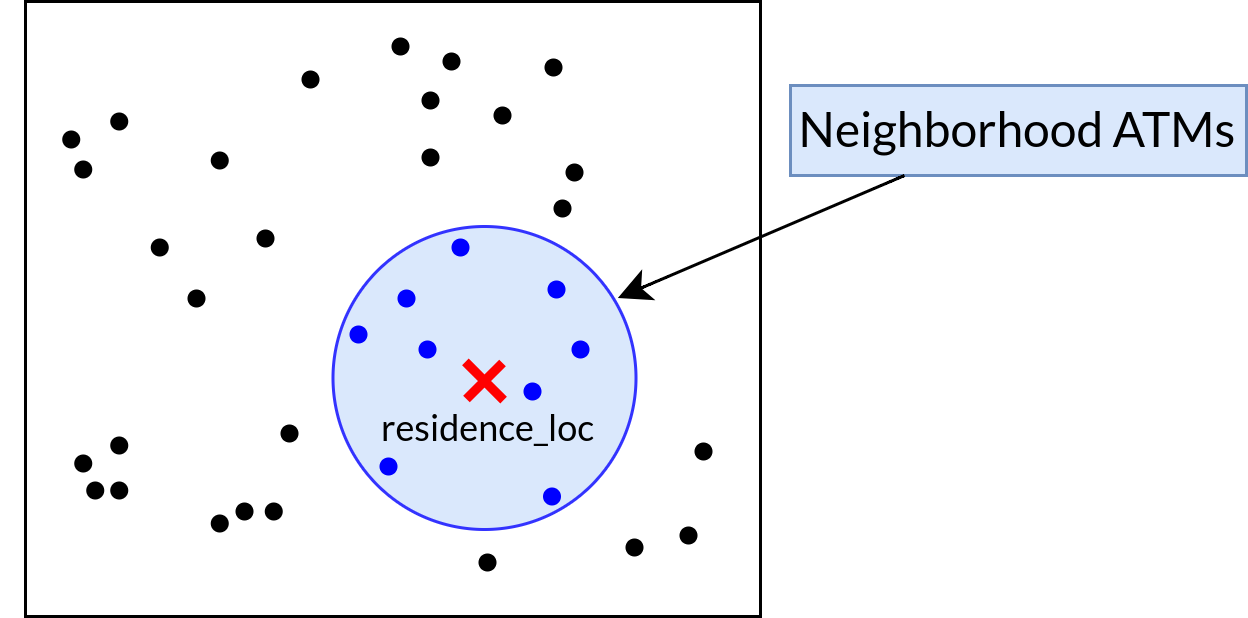
\includegraphics[scale=1.1]{images/1-DataModel/tx-generation-1-named.png}
              \caption{\texttt{Neighborhood} ATM subset}
            \end{figure}
    
        \item \textbf{Random selection}: The \texttt{ATM\_subset} is built by randomly selecting $|\texttt{ATM\_subset}|$ ATMs from the stable bank dataset.
    \end{itemize}

    \item \textbf{Calculate \texttt{t\_min\_subset}} \\
    {\footnotesize\textcolor{teal}{$\texttt{t\_min\_subset} \gets \text{calculate\_t\_min\_subset(\texttt{ATM\_subset})}$}}

    \texttt{t\_min\_subset} is the minimum threshold time needed to respect between any two consecutive transactions of a card in the regular transaction set.
    
    That is, \texttt{t\_min\_subset} is the minimum time distance between the end of a transaction and the start of the next consecutive transaction of a card, needed to guarantee in order to ensure that the constraint (I) is respected on the generation of the regular transactions set.
    
    $$\texttt{t\_min\_subset} = \frac{\texttt{max\_distance\_subset}}{\texttt{REGULAR\_SPEED}}$$

    To calculate it, we take the time needed to traverse the maximum distance between any pair of ATMs of the \texttt{ATM\_subset}: \texttt{max\_distance\_subset} at an assumed speed that any two locations can be traveled in the case of regular transaction scenarios: \texttt{REGULAR\_SPEED}.

    \item \textbf{Decide the number of transactions to be generated \texttt{num\_tx}}\\
    {\footnotesize \textcolor{teal}{$\texttt{num\_tx} \gets \text{decide\_num\_tx()}$}}
    
    Based on the behavior of the card, we decide the number of transactions \texttt{num\_tx} to generate for the card for the defined days time interval $[\texttt{START\_DATE}, \texttt{START\_DATE} + \texttt{NUM\_DAYS}]$:

    $$\texttt{num\_tx} \sim \text{Poisson}(\lambda = \texttt{ops\_day} * \texttt{NUM\_DAYS})$$ where \texttt{ops\_day} is the sum of the average number of all the kinds of operations per day of the behavior of the card: 
    $$\texttt{ops\_day} = \texttt{withdrawal\_day} + \texttt{ deposit\_day} + \texttt{ inquiry\_day} + \texttt{ transfer\_day}$$

    \item \textbf{Distribution of the \texttt{num\_tx} transaction times} \\
     {\footnotesize \textcolor{teal}{$T \gets \text{distribute}(\texttt{num\_tx}, \texttt{t\_min\_subset})$}}
    
    Along the selected time interval $[\texttt{START\_DATE}, \texttt{START\_DATE} + \texttt{NUM\_DAYS}]$ we do a random uniform distribution of the \texttt{num\_tx} transaction times. $T$ contains the list of all the the \texttt{start} and \texttt{end} times tuples for each of the \texttt{num\_tx} transactions, respecting the constraint (I) in order to guarantee that, no two consecutive transactions $tx_i$ and $tx_{i+1}$ performed in any of the ATMs of the \texttt{ATM\_subset} are at a time distance lower than \texttt{t\_min\_subset}. Specifically, the transaction times are generated guaranteeing:

    $$tx_i.\texttt{end} + \texttt{t\_min\_subset} < tx_{i+1}.\texttt{start} \ \forall i \in [1,\texttt{num\_tx})$$

    The \texttt{end} time of a transaction is assigned a shifted time difference with respect to the \texttt{start} time. In particular:

    $$
    \texttt{end} = \texttt{start} + \texttt{time\_difference}
    $$

    where:

    $$\texttt{time\_difference} \sim \mathcal{N}(\texttt{MEAN\_DURATION},\,\texttt{STD\_DURATION})$$ with the corrections:

    $$
    \texttt{time\_difference} =
    \begin{cases} 
        \texttt{MEAN\_DURATION} & \text{if } \texttt{time\_difference} < 0 \\
        \texttt{MAX\_DURATION} & \text{if } \texttt{time\_difference} > \texttt{MAX\_DURATION} \\
        \texttt{time\_difference} & \text{otherwise}
    \end{cases}
    $$

\fmc{TODO: PONER UN DIBUJITO!, explicar lo del checking de los fitting holes? --> yo creo que esto ya no es necesario... demasiado detalle}
\fmc{TODO: Explicar la variante (del generador simplificado \texttt{txGenerator-simplified.py}) en el que este distribute\_tx se cambia de tal forma que: with random order (like original version) if num holes/2 > needed holes, otherwise we introduce the transactions ordered in the time interval increasingly ordered one after
the other}

    \item \textbf{Decision on the specific values of each transaction properties:}
    Once all the previous steps are done, the specific values for the properties of each of the \texttt{num\_tx} transactions can be decided (this corresponds to the lines 7-15 in the algorithm pseudocode \ref{alg:regular-tx-generator}). Therefore for each of the transactions:
    \begin{itemize}
        \item \textbf{Link to a random ATM of the \texttt{ATM\_subset}}\\
        {\footnotesize \textcolor{teal}{$\texttt{ATM}_{i} \sim \texttt{ATM\_subset}$}}
        \item \textbf{Obtain its corresponding \emph{start} and \emph{end} time property values from the $T$ time distribution}\\
        {\footnotesize \textcolor{teal}{$\texttt{start}_{i} \gets t_i.start$, }}
        {\footnotesize \textcolor{teal}{$\texttt{end}_{i} \gets t_i.end$}}
        \item \textbf{Decide on the type of transaction}\\
        {\footnotesize \textcolor{teal}{$\texttt{type}_{i} \gets \text{getType()}$}}
        
        For each of the \texttt{num\_tx} transactions, the transaction \emph{type} is decided randomly assigning a transaction \emph{type} given a probability distribution constructed from the card behavior:
        
        $$
        \begin{cases}
          P(\texttt{type} =  \texttt{withdrawal}) = \frac{\texttt{withdrawal\_day}}{\texttt{ops\_day}} \\[8pt]
          P(\texttt{type} =  \texttt{deposit}) = \frac{\texttt{deposit\_day}}{\texttt{ops\_day}} \\[8pt]
          P(\texttt{type} = \texttt{inquiry}) = \frac{\texttt{inquiry\_day}}{\texttt{ops\_day}} \\[8pt]
          P(\texttt{type} =  \texttt{transfer}) = \frac{\texttt{transfer\_day}}{\texttt{ops\_day}} 
        \end{cases}
        $$

        where again, \texttt{ops\_day} is the sum of the average number of all the kinds of operations per day of the behavior of the card: 
        $$\texttt{ops\_day} = \texttt{withdrawal\_day} + \texttt{ deposit\_day} + \texttt{ inquiry\_day} + \texttt{ transfer\_day}$$

        \item \textbf{Assign a transaction \emph{amount}}\\
        {\footnotesize \textcolor{teal}{$\texttt{amount}_{i} \gets  \text{getAmount(}\texttt{type}_{i}\text{)}$}}
          
        The transaction \emph{amount} is assigned depending on the \emph{type} of the current transaction, based on the card behavior properties:
            
          $$
          \begin{cases}
            \mathcal{N}(\texttt{amount\_avg\_withdrawal},\, \texttt{amount\_std\_withdrawal}) & \text{if } \texttt{type} = \texttt{withdrawal} \\[10pt]
            
            \mathcal{N}(\texttt{amount\_avg\_deposit},\, \texttt{amount\_std\_deposit}) & \text{if } \texttt{type} = \texttt{deposit} \\[10pt]
        
            0 & \text{if } \texttt{type} = \texttt{inquiry} \\[10pt]
            
            \mathcal{N}(\texttt{amount\_avg\_deposit},\, \texttt{amount\_std\_transfer}) & \text{if } \texttt{type} = \texttt{transfer}
          \end{cases}
          $$
        
          $$
          \text{If } \texttt{amount} < 0, \text{ then re-draw from } U(0, 2 \cdot \texttt{amount\_avg\_type}).
          $$
        
          with \texttt{amount\_avg\_type} as \texttt{amount\_avg\_withdrawal}, \texttt{amount\_avg\_deposit} or \texttt{amount\_avg\_deposit} depending on the respective transaction \texttt{type}.   
    \end{itemize}
\end{enumerate}

An example of a transaction data item can be seen in \ref{csv:transaction}, where both the 
interaction opening and interaction close of the \emph{transaction\_id} 2804 can be observed.
\begin{center}
\lstset{style=csvStyle}
\begin{lstlisting}[caption={Example of transaction-all.csv}, label={csv:transaction}]
transaction_id,number_id,ATM_id,transaction_type,transaction_start,
transaction_end, transaction_amount
2804,c-NIGER-148,NIGER-40,0,2018-04-01 00:00:47,,
2804,c-NIGER-148,NIGER-40,0,2018-04-01 00:00:47,2018-04-01 00:04:43,26886.73
\end{lstlisting}
\end{center}

\fmc{TODO: SIGO AQUÍ!}
\textcolor{red}{\rule{\linewidth}{0.5mm}}
\fmc{TODO: Explain the simplified version of the txGenerator...:}
\textcolor{red}{For the medium size experiments (500000 cards), to generate the stream of tx, we needed to simplify this process in order to be able to generate a stream in a feasible amount of time. In particular we used the simplifed version of the \texttt{txGenerator.py}: \texttt{txGenerator-simplified.py} $\rightarrow$ with a random ATM-subset instead of a closest to client ATM-subset. Also variation on the transaction distribution times, with random order (like original version) if $num\_holes / 2 > needed\_holes$, otherwise we introduce the transactions ordered in the time interval increasingly ordered one after the other.}

\textcolor{blue}{To do the generation of the synthetic set of transactions we created the Python program \texttt{transactionGenerator.py}. On it we need to specify the value of the parameters needed to customise the generation of the set of transactions.}

\textcolor{red}{\rule{\linewidth}{0.5mm}}
\begin{itemize}
  \item Selection of ATMs:
  \begin{itemize}
    \item \textcolor{green}{$\Rightarrow$} Neighborhood / Closed ATM subset.
    \item Random walk. To do the selection of the sequence of ATMs for the generated transactions.
  \end{itemize}
  \item Distribution of the transactions along time:
  \begin{itemize}
    \item \textcolor{green}{$\Rightarrow$} Uniform distribution.
    \item \textcolor{blue}{$\Rightarrow$ (Consider the possibility)} Poisson process distribution.
  \end{itemize}
  \item Other options:
  \begin{itemize}
    \item Random walk for both the ATM and the transaction time selection, in the same algorithm together.
  \end{itemize}
\end{itemize}

\textcolor{red}{TODOS:
\begin{itemize}
\item Cambiar/Actualizar dibujos
\item Poner lista de params y explicar (tabla) como y qué se puede configurar
\item Anomalous generator:
\begin{itemize}
  \item NO-Overlapping assumption - Explain
  \item Any type of tx to produce the fraud -> does not matter the type for the FP1.
\end{itemize}
\end{itemize}
}
\textcolor{red}{\rule{\linewidth}{0.5mm}}

\paragraph{Anomalous Transaction Set\\\\}

After the generation of regular transactions we perform an injection of transactions to produce anomalous scenarios. The injection is taylored depending on the specific kind of 
anomalous scenarios that we want to produce. In what follows we explain the injection process depending on each of the types of frauds that we have considered.

\paragraph{Fraud Pattern I}

To produce anomalous scenarios related to this type of fraud, we produce the injection
of transactions that will produce the satisfaction of this fraud pattern. In other words,
we inject transactions that violate the minimum \emph{time-distance} constraint between transactions performed with the same card. Therefore, as we can see in Figure \ref{img:anomalous-type-1}, if we consider a set of regular transacions for a certain card, where $y_1$ and $y_2$ are regular consecutive transactions, we will introduce an anomalous transaction $a_{12}$ such that: 

$$(y_1.\texttt{ATM\_id} \ne a_{12}.\texttt{ATM\_id}) \land (a_{12}.\texttt{start} - 
y_1.\texttt{end} < T_{min}(y_1.\texttt{ATM\_loc}, a_{12}.\texttt{ATM\_loc}))$$

where \texttt{ATM\_loc} is the tuple of coordinates (loc\_latitude,loc\_longitude) of the corresponding ATM. This injection will produce an anomalous scenario of this kind of fraud with at least the $y_1$ previous transaction. Note that, it could possibly trigger more anomalous fraud scenarios with the subsequent transactions ($y_2$ and on...).

\begin{figure}[H]
    \centering
    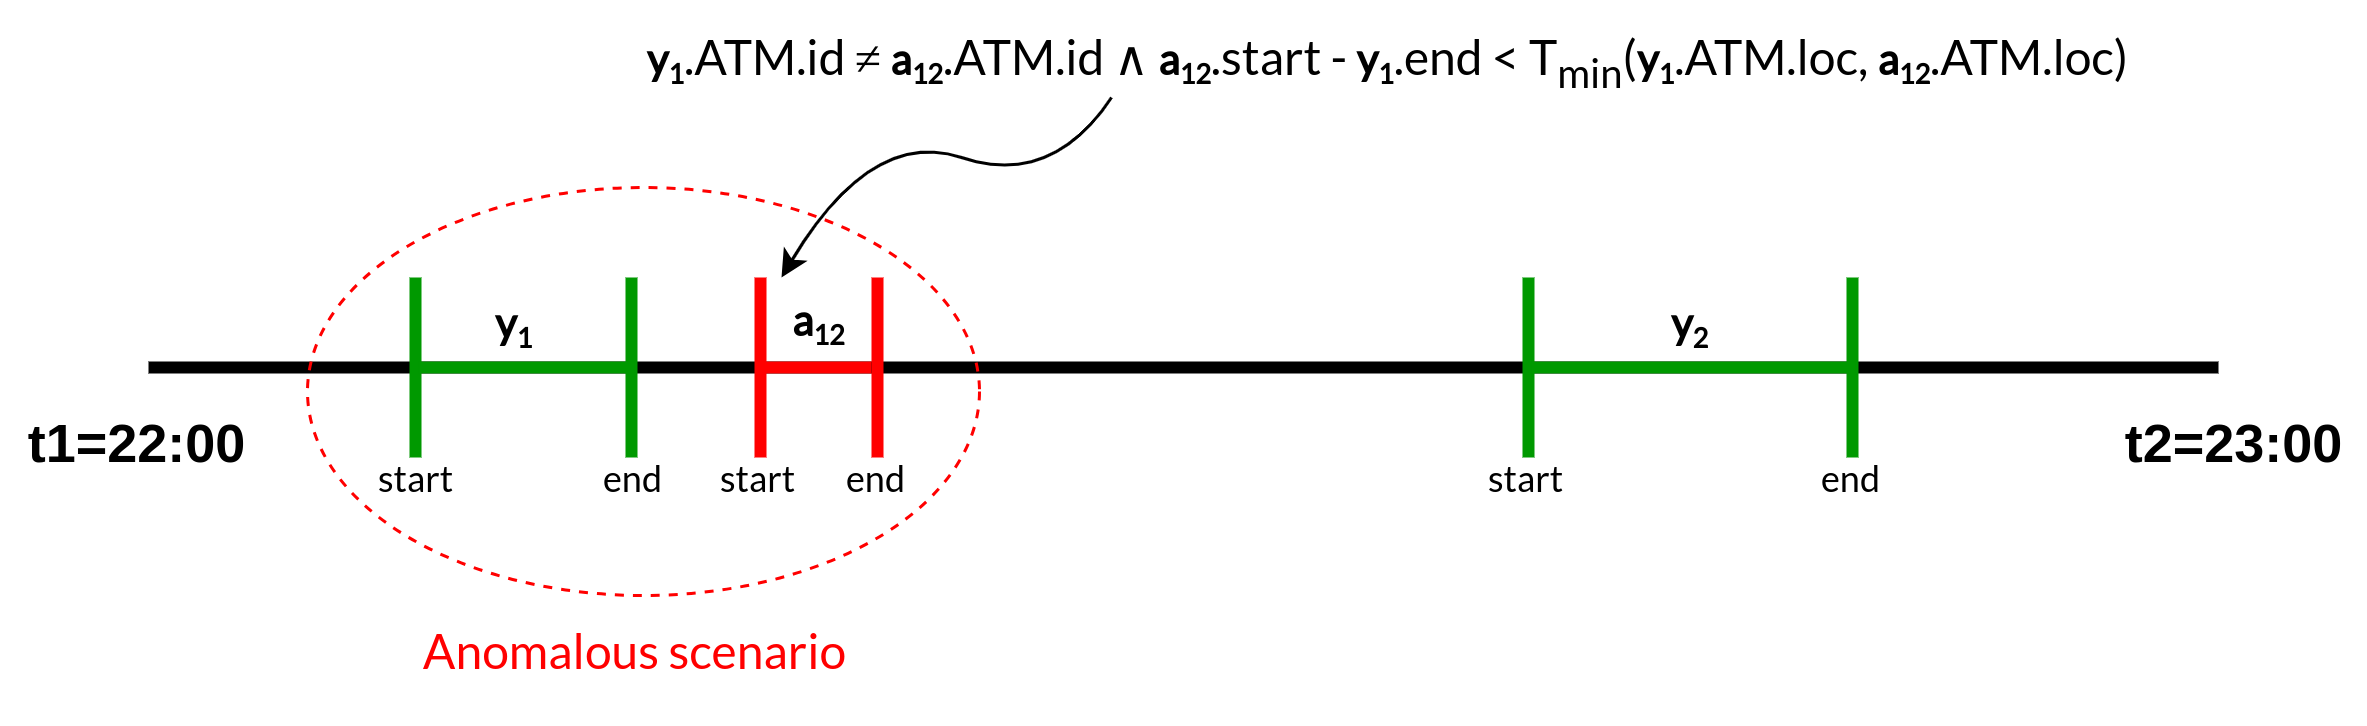
\includegraphics[width=\textwidth]{images/1-DataModel/tx-generation.png}
    \caption{Creation of anomalous scenario - type I}
    \label{img:anomalous-type-1}
\end{figure}

Some assumptions related with the generation of anomalous transactions for this kind of fraud pattern are:
\begin{itemize}
  \item \textbf{Overlapping of transactions is not possible}:
  Appart from guaranteeing that this injection causes at least one anomalous scenario, we also respect the additional constraint of ensuring that the anomalous transaction injected does not cause overlapping with any of the transactions, in particular neither with the previous nor the next one. \textcolor{orange}{This constraint is added based on the assumption that the bank itself does not allow to open a transaction whenever another one is still open.} Therefore considering that $a_{12}$ is the anomalous injected transaction in between the regular consecutive transactions $y_1$ and $y_2$, when generating $a_{12}$ we guarantee that:
  $$
  \begin{cases}
    a_{12}.\texttt{start} > y_{1}.\texttt{end} \\
    a_{12}.\texttt{end} < y_{2}.\texttt{start}
  \end{cases}
  $$
  \item \textbf{There are no two consecutive anomalous transactions}: For simplicity in our practical purposes, we do the generation of anomalous transactions for this kind of fraud pattern assuming that an anomalous transaction can only be in between two regular consecutive transactions, so that we do not consider the case of the injection of two or more consecutive anomalous transactions for this kind of fraud. See Figure \ref{img:anomalous-type-1-insertion-points}.
  \begin{figure}[H]
    \centering
    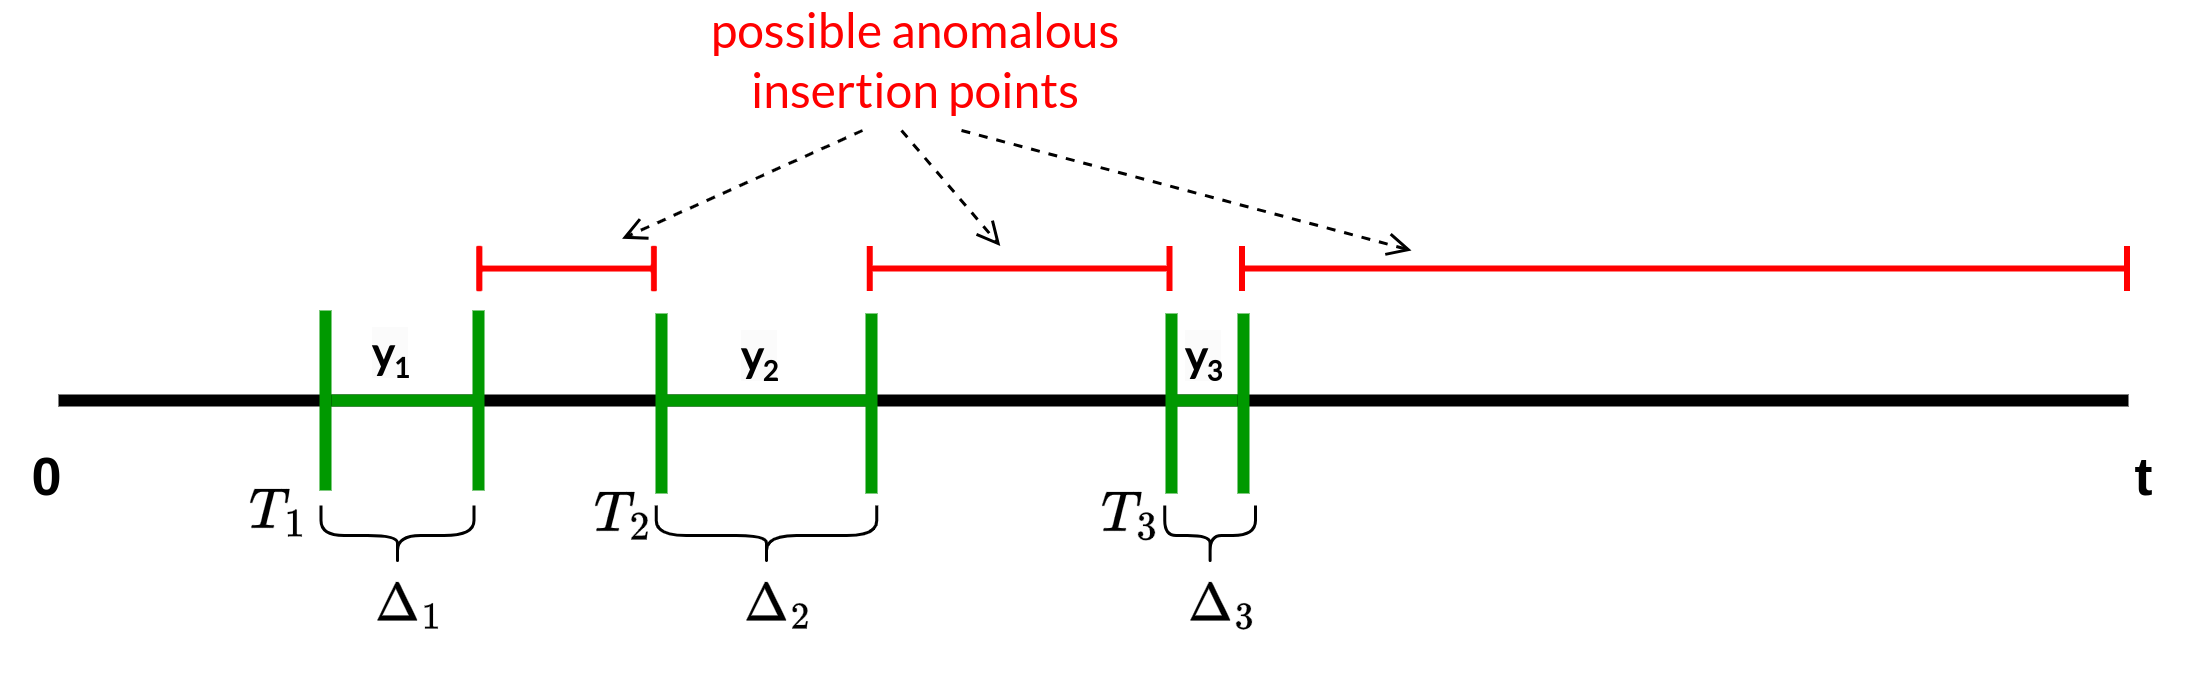
\includegraphics[width=\textwidth]{images/1-DataModel/tx-generation-anomalous-1.png}
    \caption{Considered possible injection points of anomalous transactions of fraud type I}
    \label{img:anomalous-type-1-insertion-points}
  \end{figure}  
\end{itemize}

We generate $\texttt{ANOMALOUS\_RATIO\_1} * \texttt{num\_tx}$ anomalous transactions for each of the cards related with the fraud pattern I, where $\texttt{ANOMALOUS\_RATIO\_1} \in [0,1]$ defines the ratio of anomalous transactions of this kind over the total number of regular transactions \texttt{num\_tx} for each of the cards. In Algorithm \ref{alg:anomalous-tx-generator-1} we describe at a high level the process of the generation of anomalous transactions for this kind of fraud pattern. 


\textcolor{red}{Preconditions:
\begin{itemize}
  \item ATMsubset, and the compl. are given by param, from the tx regular generator
\end{itemize}
}

\begin{algorithm}[H]
  \small
  $\textbf{introduceAnomalous}(\texttt{ATM\_subset}, \overline{\texttt{ATM\_subset}})$
  \begin{algorithmic}[1]
  \STATE $\texttt{num\_anomalous} \gets \texttt{num\_tx} * \texttt{ANOMALOUS\_RATIO\_1}$
  \STATE $i \gets 0$
  \WHILE{$i < \texttt{num\_anomalous}$}
      \STATE $\texttt{ATM}_{i} \sim \overline{\texttt{ATM\_subset}}$
      \STATE $prev_i, next_i \gets \text{randomUniquePosition(\texttt{num\_tx})}$
      \STATE $t_i \gets \text{getTime}(prev_i, next_i)$
      \STATE $\texttt{start}_{i} \gets t_i.start$
      \STATE $\texttt{end}_{i} \gets t_i.end$
      \STATE $\texttt{type}_{i} \gets \texttt{getRandomType()}$
      \STATE $\texttt{amount}_{i} \gets \texttt{getAmount()}$
      \STATE $\texttt{id}_{i} \gets \texttt{id}; \ \texttt{id} \gets \texttt{id} + 1$
      \STATE $\texttt{createTransaction}(\texttt{id}_{i}, \texttt{ATM}_i, \texttt{start}_{i},\texttt{end}_{i}, \texttt{type}_{i}, \texttt{amount}_i)$
      \STATE $i \gets i + 1$
  \ENDWHILE
  \end{algorithmic}
  \caption{Introduction of Anomalous Transactions for Fraud Pattern I}
  \label{alg:anomalous-tx-generator-1}
\end{algorithm}


\begin{enumerate}
  \item \textbf{Assignment of ATMs not belonging to the \texttt{ATM\_subset}}: the anomalous transactions are linked to ATMs that are part of the complementary of the \texttt{ATM\_subset}.
  \item \textbf{Each anomalous transaction has a unique insertion position}: As described previously, we do not allow the case of two or more consecutive anomalous transactions injection. Each anomalous transaction occupies a unique position among all the possible injection positions defined by the set of regular transactions generated for the card. As it can be seen on Figure \ref{img:anomalous-type-1-insertion-points}, considering that we have three regular transactions, we will consider three unique possible insertion points for the anomalous transactions. The procedure of assigning a unique insertion position for each anomalous transaction to be generated is achieved with the function \text{randomUniquePosition(\texttt{num\_tx})}, that given the number of regular transactions of the card \texttt{num\_tx} returns the previous and the next regular transaction to the assigned unique position.
  \item \textbf{Assign transaction times such that respecting the needed time constraints}: in particular there are two time constraints to be satisfied:
  \begin{itemize}
    \item Production of fraud pattern with prev\_i
    \item No overlapping with prev\_i nor with next\_i
  \end{itemize}
  This is summarized in the pseudocode as the procedure getTime(prev\_i, next\_i), which returns $t_i$, as the tuple of (\texttt{start},\texttt{end}) times.
  \item \textbf{Random transaction type}
  \item \textbf{Arbitrary amount}
 
\end{enumerate}

\fmc{Poner otras opciones consideradas? - ver texto comentado justo debajo}

\begin{comment}
\subsubsection{ATM closed subset + Poisson Process}

\begin{tcolorbox}
  \begin{itemize}
    \item[$\rightarrow$] \textbf{ATM selection}: Closed ATM subset.
    \item[$\rightarrow$] \textbf{Time distribution}: Poisson process distribution of $num\_tx$ 
    transactions for each of the cards.
  \end{itemize}
\end{tcolorbox}

Generate $\texttt{num\_tx}$ transactions for a selected period of time $\texttt{t}$.
Distribution following a Poisson process distribution along $[0,t]$.
\begin{itemize}
    \item[$\bullet$] $\lambda=\texttt{avg\_tx}$ on a day for the client if $\texttt{t = 24h}$. Otherwise, 
    decide a specific $\lambda$ for the considered $\texttt{t}$.
    \item[$\bullet$] Inter-arrival times $X_1, X_2, \cdots$ are distributed following an exponential distribution:
    $X_i \sim \text{Exp}(\lambda)$. They represent the time elapsed between two of these events, e.g. $X_2$ represents the time elapsed between the first and the second arrival. Note that in this case, since we need to respect the minimum required time between two consecutive 
    transactions ($t_{min}$) so to avoid introducing anomalous undesired scenarios, we have to impose
    that: $X_i \geq \Delta_{i-1} + t_{min}, \forall X_i$, where:

    \begin{itemize}
      \item[$\circ$] $X_{i}$: time elapsed between the $i$-$1$ and $i$-th transaction.
      \item[$\circ$] $\Delta_{i-1}$: time duration of the $i$-$1$ transaction. This duration will 
      be upper bounded by $\Delta_{max}$, which will be considered the maximum possible duration of a transaction.
      \item[$\circ$] $t_{min}$: minimum calculated time distance between any 2 consecutive transactions of the client.
  \end{itemize}

    With these interarrival times, we obtain the arrival times $T_i$. Note that they are not independent, in particular:
    $T_1 \leq T_2 \leq T_3 \cdots$.

    Therefore, to generate the Poisson process with rate $\lambda$:
    \begin{enumerate}
      \item Generate i.i.d. random variables $X_1, X_2, \cdots$ where $X_i \sim \text{Exp}(\lambda)$.
      \item Obtain the arrival times as:
        \begin{itemize}
          \item $T_1 = X_1$
          \item $T_2 = X_1 + X_2$
          \item $T_3 = X_1 + X_2 + X_3$
          \item $\cdots$
        \end{itemize}
    \end{enumerate}

    Note that, having imposed the previous we will have that:
    \begin{equation}
      \begin{cases}
        T_i = T_{i-1} + X_i \\
        X_i \geq \Delta_{max} + t_{min}
      \end{cases}\forall X_i \
    \end{equation}

    which implies that:
    
    \begin{equation}
      T_i \geq T_{i-1} + \Delta_{max} + t_{min}, \forall X_i
    \end{equation}
    
\end{itemize}
\begin{figure}[H]
    \centering
    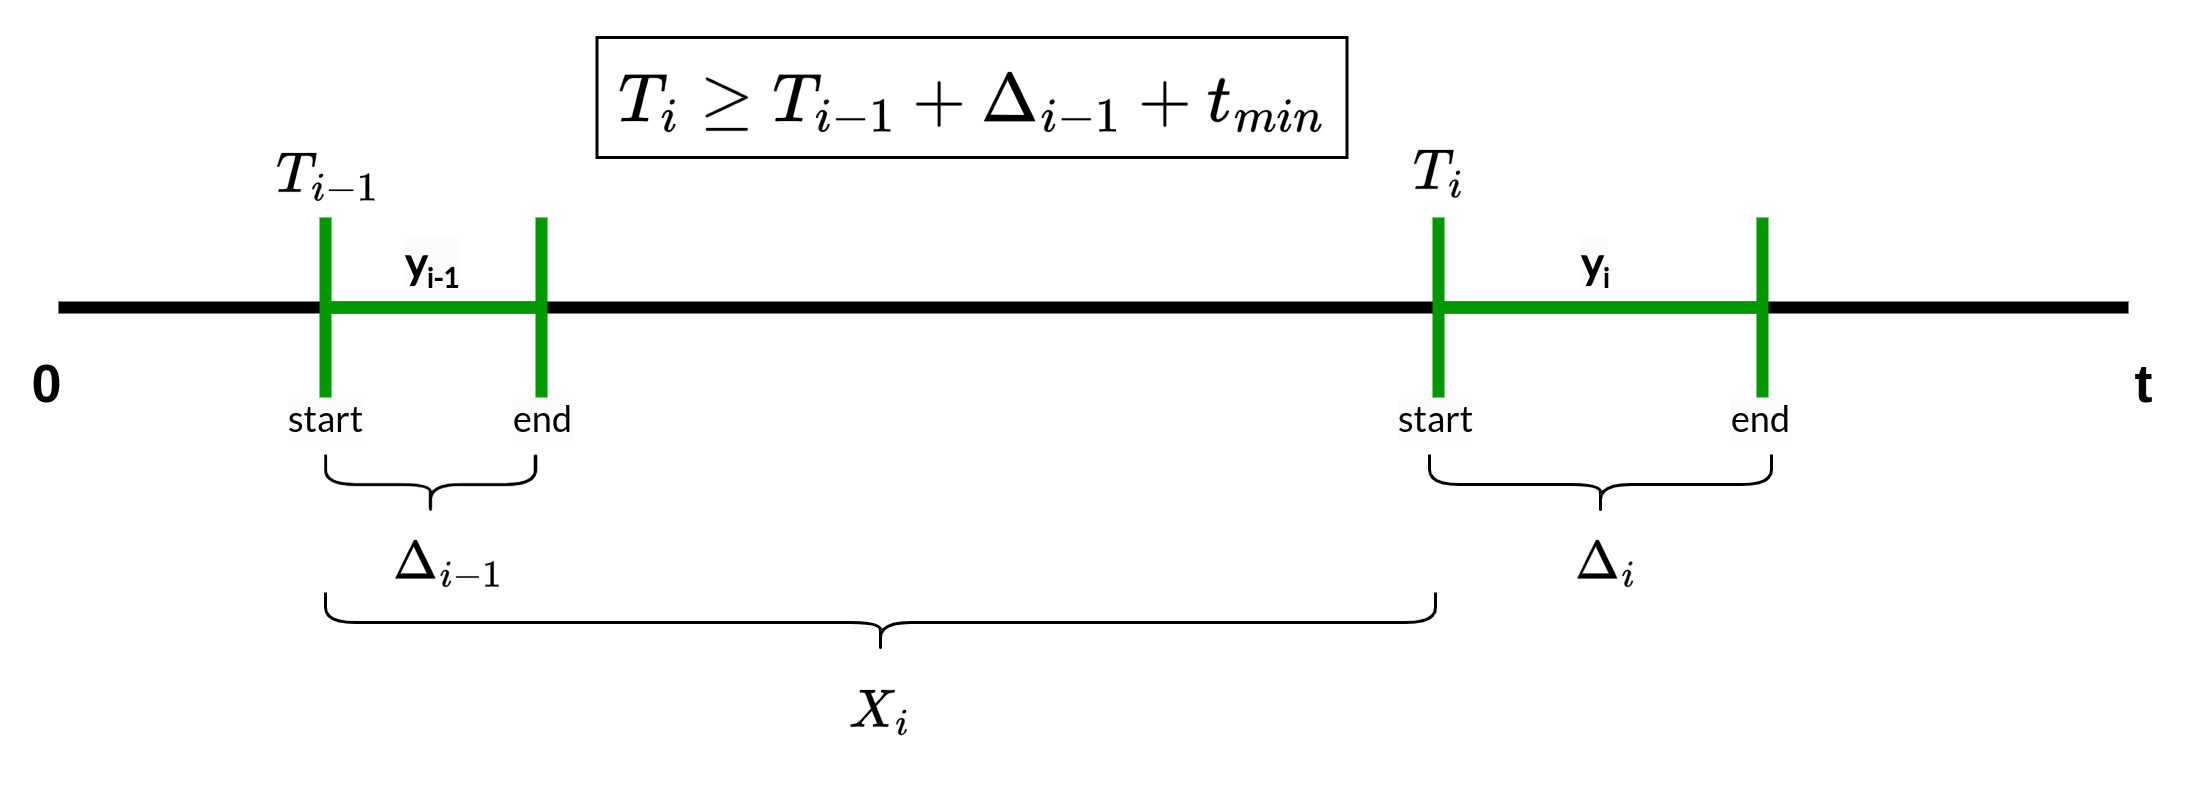
\includegraphics[scale=0.55]{images/tx-generation-dist-corrected.png}
    \caption{Schema of the interarrival and arrival event times on the poisson process.}
\end{figure}


References:

\begin{itemize}
  \item \href{https://www.probabilitycourse.com/chapter11/11_1_2_basic_concepts_of_the_poisson_process.php}{Poisson process modeling - Theoric description}
  \item \href{https://www.probabilitycourse.com/chapter14/Chapter_14.pdf}{Poisson process modeling - Python implementation}
  \item \href{https://timeseriesreasoning.com/contents/poisson-process/}{Less formal explanation with Python code}
  \item \href{https://www.math.wsu.edu/faculty/genz/416/lect/l05-45.pdf}{More theory}
  \item \href{https://en.wikipedia.org/wiki/Poisson_point_process}{Wikipedia entry}
\end{itemize}

\subsubsection{Random Walk / Markov Chain}

Idea is to model the sequence of transactions for each of the clients as a markov chain through the
network of ATMs. The network is a fully-connected graph with ATMs as nodes and edges are
weighted with the distance between each pair of ATMs as weights.

The idea is to obtain the sequence of transactions for each client as a markov chain, in which,
for each step a transaction is generated in that specific ATM node, at a certain datetime 
respecting the constraint of the minimum time distance with the previous transaction, so 
that no undesired anomalous fraud scenarios are produced. \\ 

Some considerations:
\begin{itemize}
  \item Initially, we will compute the transition matrix obtaining all the respective 
  transition probabilities. The probability of transition to another ATM-node will be 
  inversely proportional to the distance to the considered ATM-node.
  \item Transition matrix $P_t$: containing, for each state, the probability of transitioning
  between states. For example, the entry $i,j$: $(P_t)_{i,j} = \mathcal{P}(X_{t+1} = j | X_t = i)$
  contains the probability of transitioning to state $j$ when being in state $i$. 
  Note that since we assume a complete graph, and also the posibility to transition 
  to the same state, all entries of this matrix will be distinct to 0: $(P_t)_{i,j} \neq 0 \  
  \forall i,j$.
  \item Finally, once $P_t$ is computed, we perform the simulation to obtain the sequence of
  transactions for the specific card/client.
\end{itemize}

References:

\begin{itemize}
\item Markov Chains
\begin{itemize}
  \item \href{https://brilliant.org/wiki/markov-chains/}{MC - Theory}
  \item \href{https://www.columbia.edu/~ks20/4703-Sigman/4703-07-Notes-MC.pdf}{Simulation of Markov Chains - Theory}
  \item \href{https://stephens999.github.io/fiveMinuteStats/simulating_discrete_chains_1.html}{MC - Implementation example}
  \item \href{https://www.youtube.com/watch?v=G7FIQ9fXl6U}{MC - Implementation video example}
\end{itemize}
\item Random Walks
\begin{itemize}
  \item Theory:
  \begin{itemize}
    \item \href{https://ieeexplore.ieee.org/abstract/document/8911513?casa_token=vznpjKL5HG0AAAAA:hNzLCxAHBk75zCDUHsswB7ImAKgilzZcOBzxaXWz_G6U8Vy-ogbei40MoZ49M-Em5tTii0Q}{RWs: A Review of Algorithms and Applications}
    \item \href{https://www.lirmm.fr/~sau/JCALM/Josep.pdf}{RWs on Graphs}
    \item \href{https://www.fi.muni.cz/usr/gruska/random18/random1808.pdf}{RW - More theory}
  \end{itemize}
  \item Implementation examples:
  \begin{itemize}
    \item \href{https://tleise.people.amherst.edu/Math365Spring2016/RmarkdownFiles/WalkOnGraph.html}{Simple RW on a Graph - Implementation example}
    \item \href{https://graphstream-project.org/doc/Algorithms/Random-walks-on-graphs/}{A RW on a graph - Implementation}
    \item \href{https://es.mathworks.com/help/econ/simulate-random-walks-through-markov-chain.html}{Simulate Random Walks Through Markov Chain - Matlab Implementation example}
  \end{itemize}
\end{itemize}
\end{itemize}
\end{comment}

\fmc{TODO: Explain the different program versions done and how to use each. 
Files generated. Show example of the csv.}


\paragraph{Transaction dataset generator: \texttt{txGenerator.py} \\\\}

To do the generation of a transaction stream dataset we developed a Python program \texttt{txGenerator.py}. The program contains some parameters used for the customization of the generated transaction stream. 

\fmc{TODO: List the parameters to configure/set up the generation of the tx stream}
% Description/list the parameters
To use it:

\begin{enumerate}
    \item Ensure to have a \texttt{csv} named directory with the \emph{csv} stable bank dataset files on which we want to simulate a transaction stream (use the bank data generator to produce it).
    \item Run \texttt{\$> python3 txGenerator.py <outputFileName>} -- \textcolor{gray}{Run with Python3.6 version or higher} -- introducing \emph{outputFileName} as an argument to name the transaction dataset files to be generated.
\end{enumerate}

The program generates a \texttt{tx} directory with the \emph{csv} files representing the transaction stream dataset:

\begin{itemize}
    \item \texttt{<outputFileName>-all.csv}: joint regular and anomalous dataset.
    \item \texttt{<outputFileName>-regular.csv}: regular transaction dataset.
    \item \texttt{<outputFileName>-anomalous.csv}: anomalous transaction dataset.
\end{itemize}


\fmc{TODO: Explicar la versión simplificada. Random ATM subset. Actualización de la función de dsitribute\_tx, = if $num\_holes / 2 \ge needed\_holes$...}
\paragraph{Transaction dataset generator: \texttt{txGenerator-simplified.py} \\\\}


\subsection{Stream ingestion}\label{exps-input-reading}

As it was already advanced in the description of the implementation of the \source \Sr stage in \ref{ContinuousQueryEngine}, the way the stream of interactions is input into the \DPATM system is of paramount importance when evaluating the performance of a real-time system like ours.

\fmc{TODO: Poner referencias a Apache Kafka/Flink... articulos relacionados con message queues para el consumo de un data stream}
\begin{itemize}
  \item \href{https://www.confluent.io/es-es/learn/apache-flink/}{Apache Flink}: distributed processing engine for stateful computation of data streams.
\end{itemize}

In a real-case scenario, the interaction/transaction events coming from the network of ATMs of the bank would be typically received in a stream manner by a message queue of the \DPATM system. However, to test our proof of concept \DPATM system, we decided to simplify this process and do a file input read of the \texttt{csv} files containing our generated simulated synthetic transaction streams. The interactions are read from these files, parsed into \texttt{Edge} data types and provided to the pipeline in different ways depending on the kind of simulation we perform. \\

For all the kinds of experiments we perform we want the reading of the input file to be the fastest possible, so to minimize the potential bottleneck derived from the I/O operation of reading a file. With this purpose, we utilized a buffered reader of the \texttt{bufio} package, which reads chunks of data into memory, providing buffered access to the file. This buffered reader was provided to a \texttt{csv} reader of the \texttt{encoding/csv} package to read the buffered stream as \texttt{csv} records.


    \begin{center}
    \lstset{style=golangStyle}
    \begin{lstlisting}[caption={\texttt{csv-bufio} reader}]
        reader := csv.NewReader(bufio.NewReader(file))
    \end{lstlisting}
    \end{center}
    
% Lectura por chunks
% chunk size = 100
% read with the help of a worker to keep reading in the background, to accelerate the reading -> explain the reason of why this
Another optimization that was done in order to be able to minimize this bottleneck on the reading of the interactions from the \texttt{csv} file, was reading by chunks the \texttt{csv} records/rows. In particular, this was done by having a \textit{worker} subprocess, implemented as an anonymous \texttt{goroutine} inside \Sr, whose task was to continuously read records from the file using the \texttt{csv-bufio} reader accumulating them in a chunk of rows that were provided through a channel to \Sr whenever they reached the defined \emph{chunkSize}. These records were read directly as \texttt{string} data types. On its side, whenever \Sr received a chunk of rows, it takes each of the rows on it, parses it to the \texttt{Edge} data type and sends it through the pipeline to the next stage. The \emph{chunkSize} was selected to be of $10^2$ rows.\\

The justification of the usage of this buffered and chunked file reading using the \texttt{encoding/csv} package with a \emph{chunkSize} of $10^2$ rows is provided with the upcoming results. On them the \texttt{encoding/csv} package performance is compared to other variants using the \texttt{apache/arrow} package with different combinations of \emph{chunkSize}. We also analyze the benefits of introducing the \textit{worker} subprocess to perform the chunked reading.\\

Some references that we utilized include: \cite{exps-input-read-go_apache_arrow, exps-input-read-apache_arrow_go_match, exps-input-read-apache_arrow_medium, exps-input-read-golang_arrow_voltrondata} are different blogs and tutorials where \texttt{Apache Arrow} is explained and where its usage with \texttt{Go} is also exemplified.
\cite{exps-chunk-by-chunk-reading} is an informal post where they experimentally showed some of the benefits of file reading in chunks.\\

% 1. comparison of csv/encoding with the other variants
First the performance of the \texttt{encoding/csv} package is compared to the \texttt{apache/arrow} package. \texttt{encoding/csv}\footnote{\url{https://pkg.go.dev/encoding/csv}} is the package provided by the \texttt{Go} standard library to decode and encode data using \texttt{csv} values format.
% describo apache/arrow - era con bufio? comprobar
\texttt{apache/arrow}\footnote{\url{https://pkg.go.dev/github.com/apache/arrow/go/arrow/csv}} is a \texttt{Go} package from the \texttt{Arrow}\footnote{\url{https://pkg.go.dev/github.com/apache/arrow/go/arrow}} platform that allows reading \texttt{csv} files in chunks of $n$ rows, called \emph{records}. An inconvenient is that \texttt{Apache Arrow} is optimized storing the data in a columnar way (by columns). So that we can not access the original $n$ rows easily, but instead the columns of these rows. And therefore, from them we will need to reconstruct the rows by taking the corresponding elements from each of the columns, given the index of the corresponding row.\\

All the compared approaches do the reading by chunks in a worker subroutine. The chunks are then provided to the main process through an internal communication channel. This intends to simulate a real implementation of the \source \Sr stage.

\begin{itemize}
  \item \texttt{apache/arrow-1}: Reading done with \texttt{apache/arrow} package. The worker performs the reading of each field of the \texttt{csv} with its corresponding data type. After reading a chunk, it is then transposed back to obtain the \texttt{Edge} type rows (as the library optimizes saving the \texttt{csv} by columns when read), and the chunk of \texttt{Edge} rows given to the main process. 
  \item \texttt{apache/arrow-2}: Reading done with \texttt{apache/arrow} package. The worker reads each field as \texttt{string} data type. After reading a chunk, it is transposed bank to row form and sent to the main process. The conversion to the corresponding \texttt{Edge} types is performed in the main process.
  \item \texttt{csv/encoding}: Reading done using the \texttt{encoding/csv} package. Row by row reading by the worker. When a chunk of rows is formed it passes it to the main process and the rows are then converted to \texttt{Edge}'s.
\end{itemize}

To perform these experiments we generated \texttt{csv} stream files of toy interactions of different sizes: $10^4$, $10^5$ and $10^6$ number of interactions (rows). For each of the sizes we compared the time it took to read the full file to each of the variants, also testing with different chunk sizes in terms of the number of rows: ranging from $10^0, 10^1, 10^2...$ up to the total number of rows of the file (maximum possible chunk size, i.e. all at once). Each of the experiments performed were run a total of 20 times to obtain stable measurements. The results can be seen in Figure \ref{img:exps-read-input-variants}. In all of the cases, the fastest approach is the variant using \texttt{encoding/csv} with chunk size \emph{chunkSize} of $10^2$ rows.\\

\begin{figure}[H]
  \centering
  \begin{minipage}{0.48\textwidth}
    \centering
    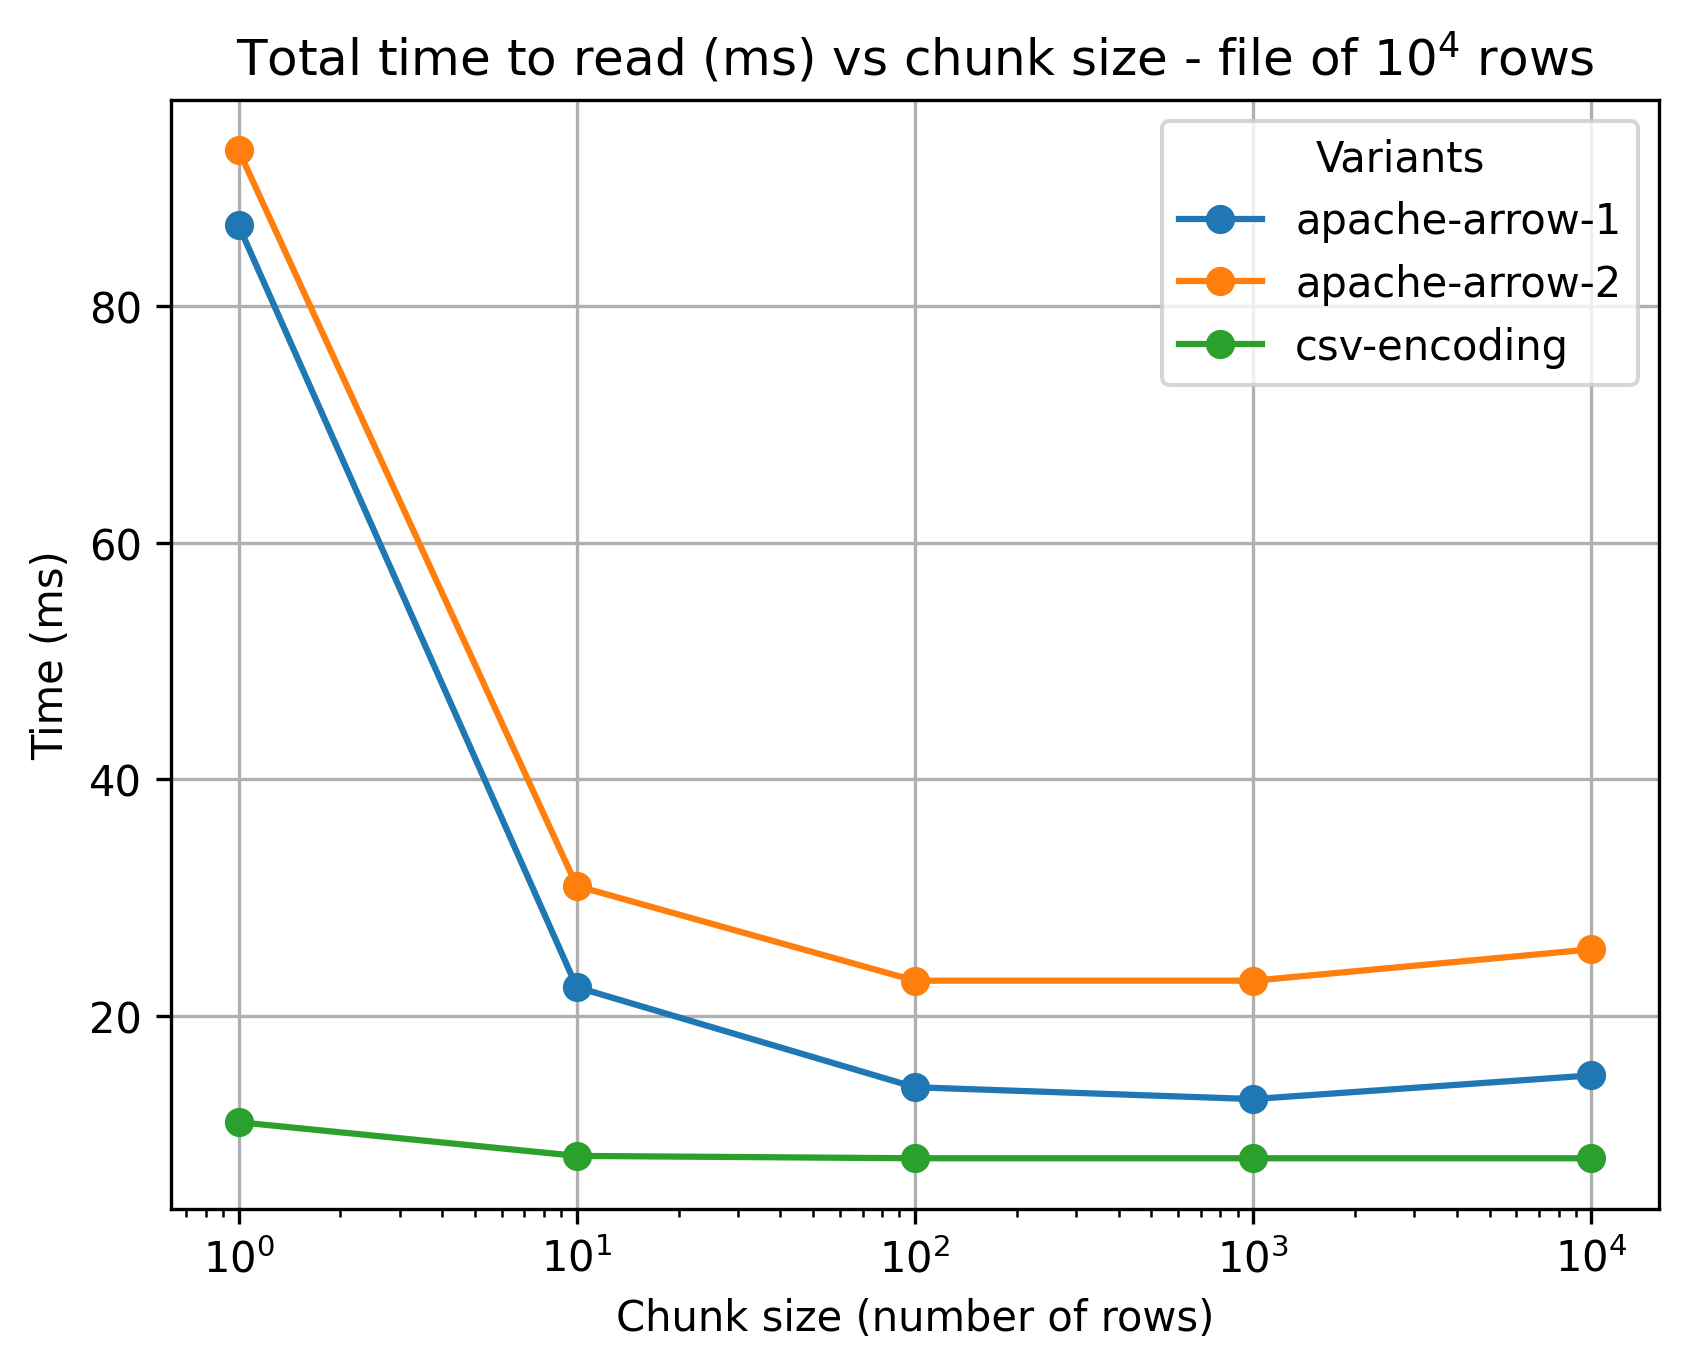
\includegraphics[scale = 0.5]{images/4-Experiments/read-input-10-4.png}
    \caption*{Test for \texttt{csv} file of size $10^4$ rows}
  \end{minipage}
  \hfill
  \begin{minipage}{0.48\textwidth}
    \centering
    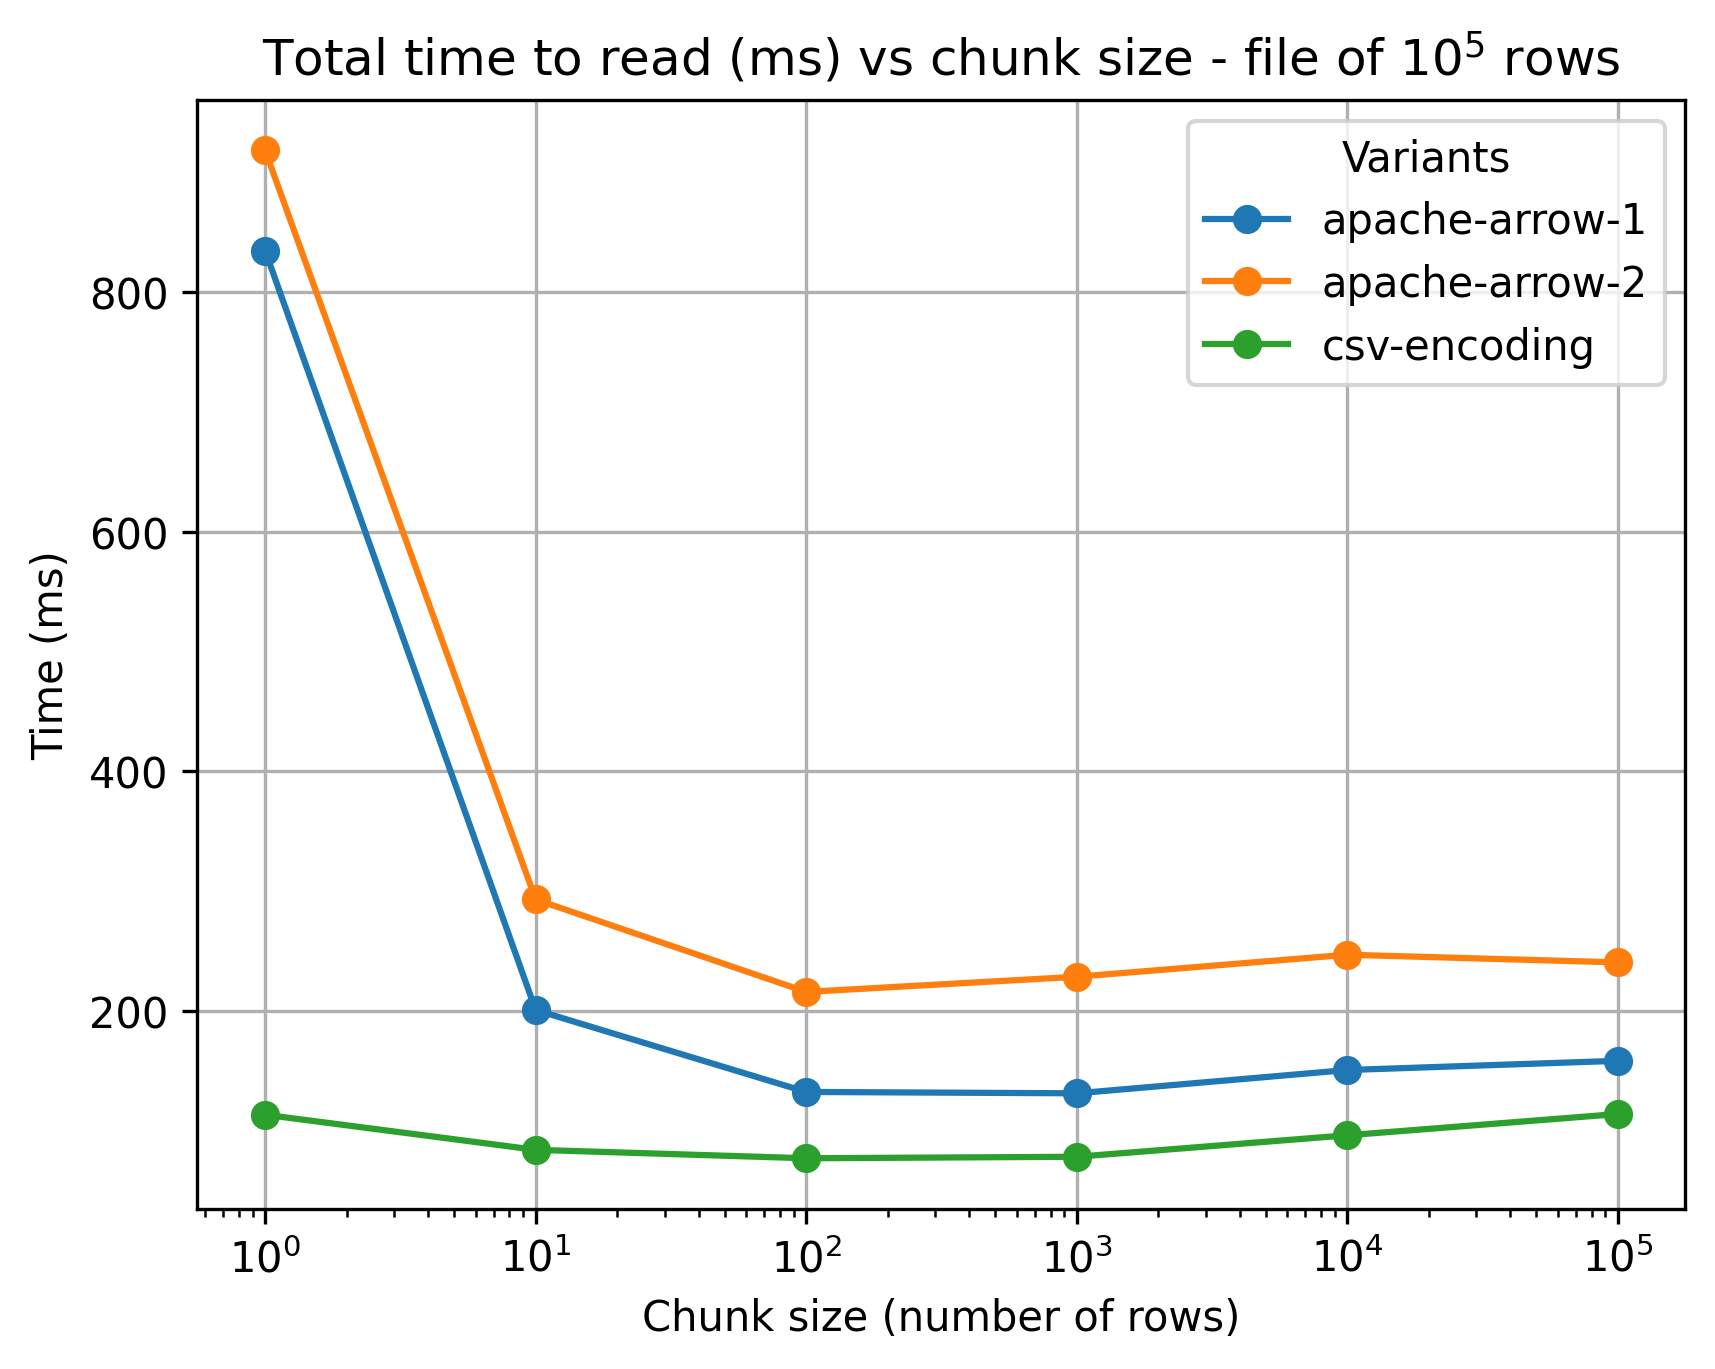
\includegraphics[scale = 0.5]{images/4-Experiments/read-input-10-5.png}
    \caption*{Test for \texttt{csv} file of size $10^5$ rows}
  \end{minipage}
  
  \vspace{0.5cm} % Add some vertical space between the rows

  \begin{minipage}{0.6\textwidth}
    \centering
    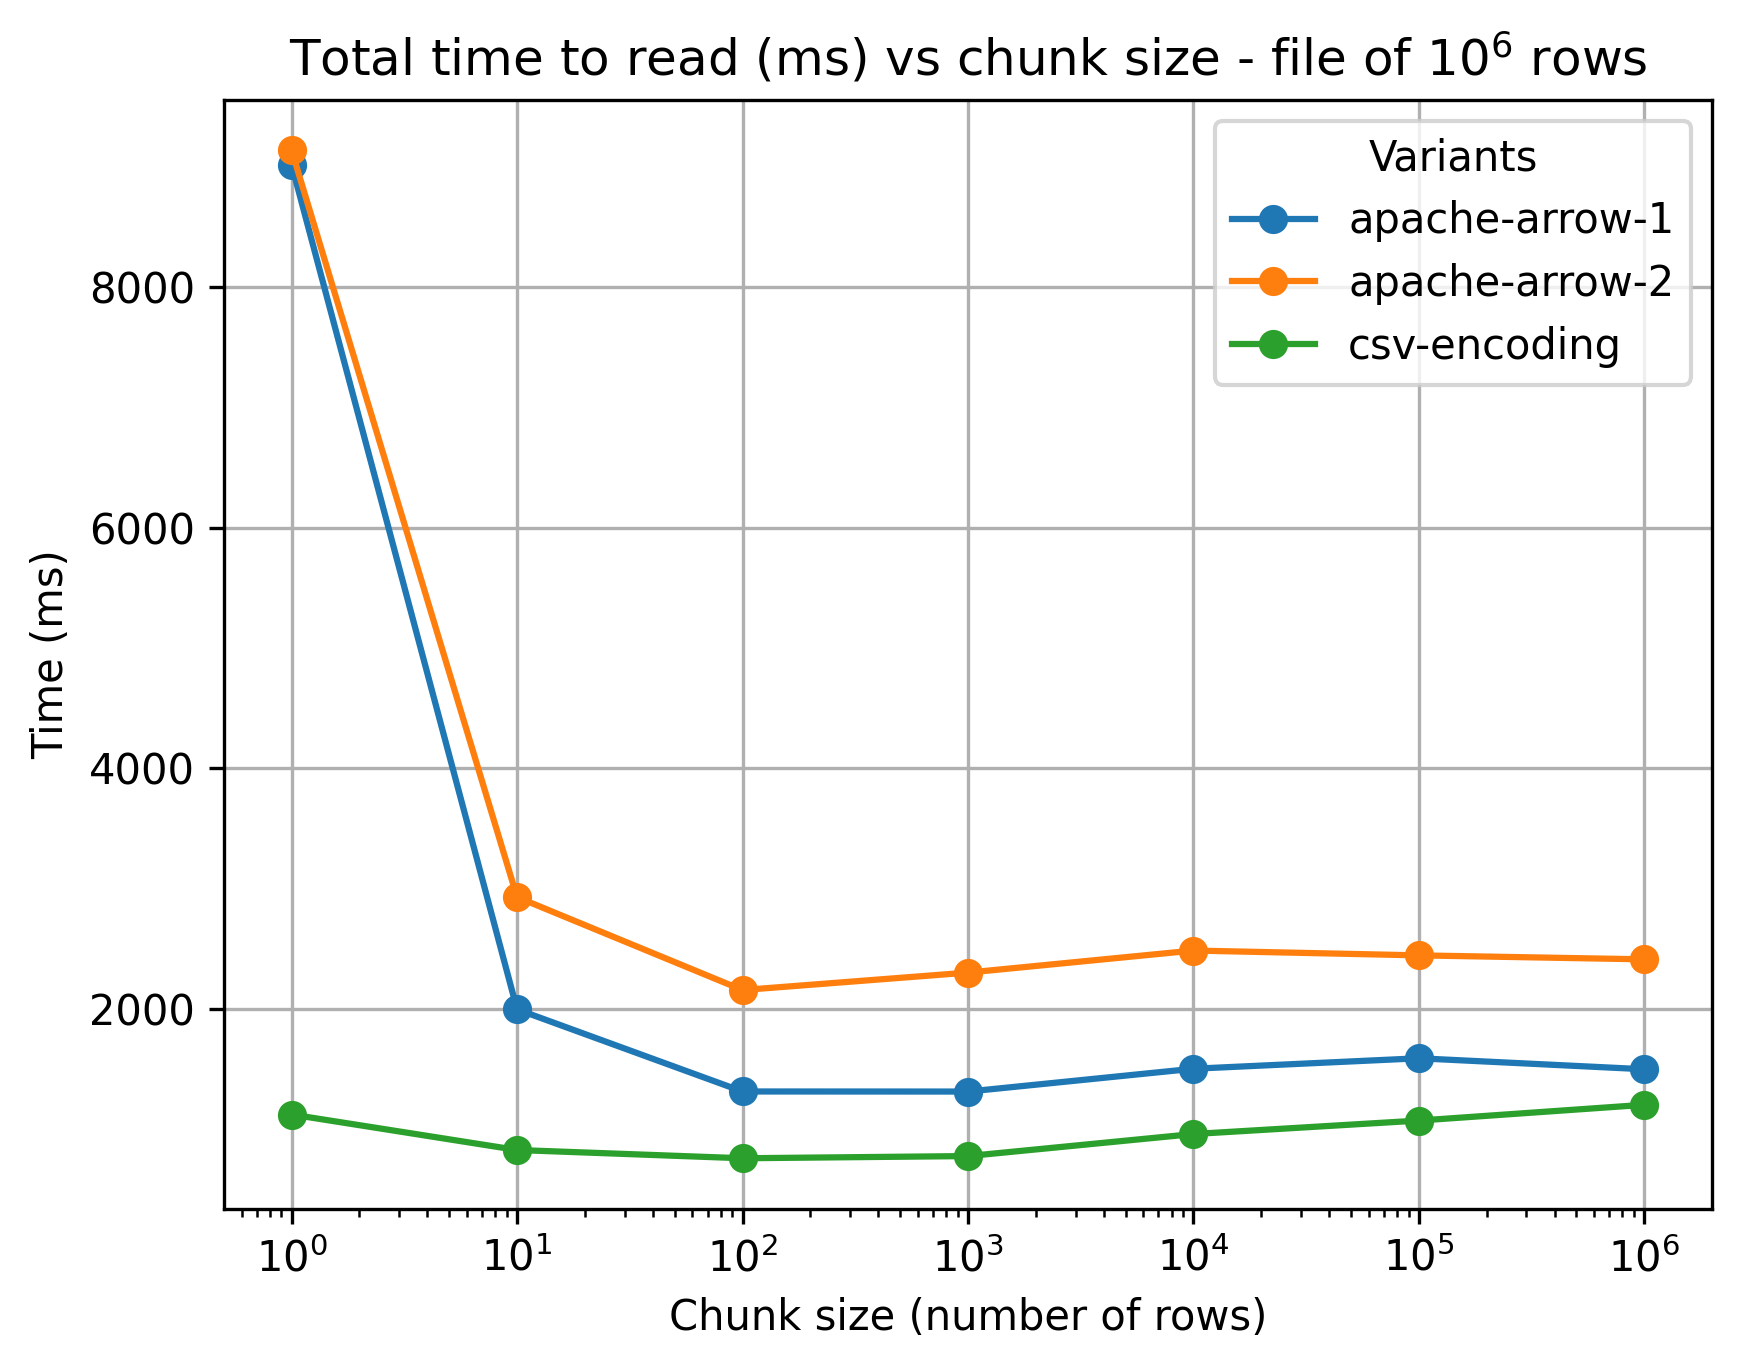
\includegraphics[scale = 0.5]{images/4-Experiments/read-input-10-6.png}
    \caption*{Test for \texttt{csv} file of size $10^6$ rows}
  \end{minipage}
  \caption{Comparison of the \texttt{apache/arrow-1}, \texttt{apache/arrow-2} and \texttt{encoding/csv} variants for reading different \texttt{csv} file sizes, using different chunk sizes.}
  \label{img:exps-read-input-variants}
\end{figure}

% 2. comparison of the benefits of no-worker vs worker with the csv/encoding
Once we decided to use the approach using the \texttt{encoding/csv} package, we performed an additional experiment in order to see if it was actually worthy to do the \emph{background} reading of the input with the worker subprocess \texttt{goroutine}. To see this we performed some experiments in which we compared the variant with worker and chunk size of $10^2$ with respect to the one without worker and without chunk reading. Again we compared the time it took to read \texttt{csv} interaction files of different sizes : from $10^4$ up to $10^6$ and $10^7$ rows/interactions. Each experiment was done 20 times to obtain stable measurements.\\

As it can be seen in Figure \ref{img:exps-csv-encoding-variants}, the differences are insignificant. Up to $10^6$ rows the variant with worker and chunk reading seems to be slightly better, although for the experiment with $10^7$ rows is the other way around.

\begin{figure}[H]
  \centering
  \begin{minipage}{0.49\textwidth}
    \centering
    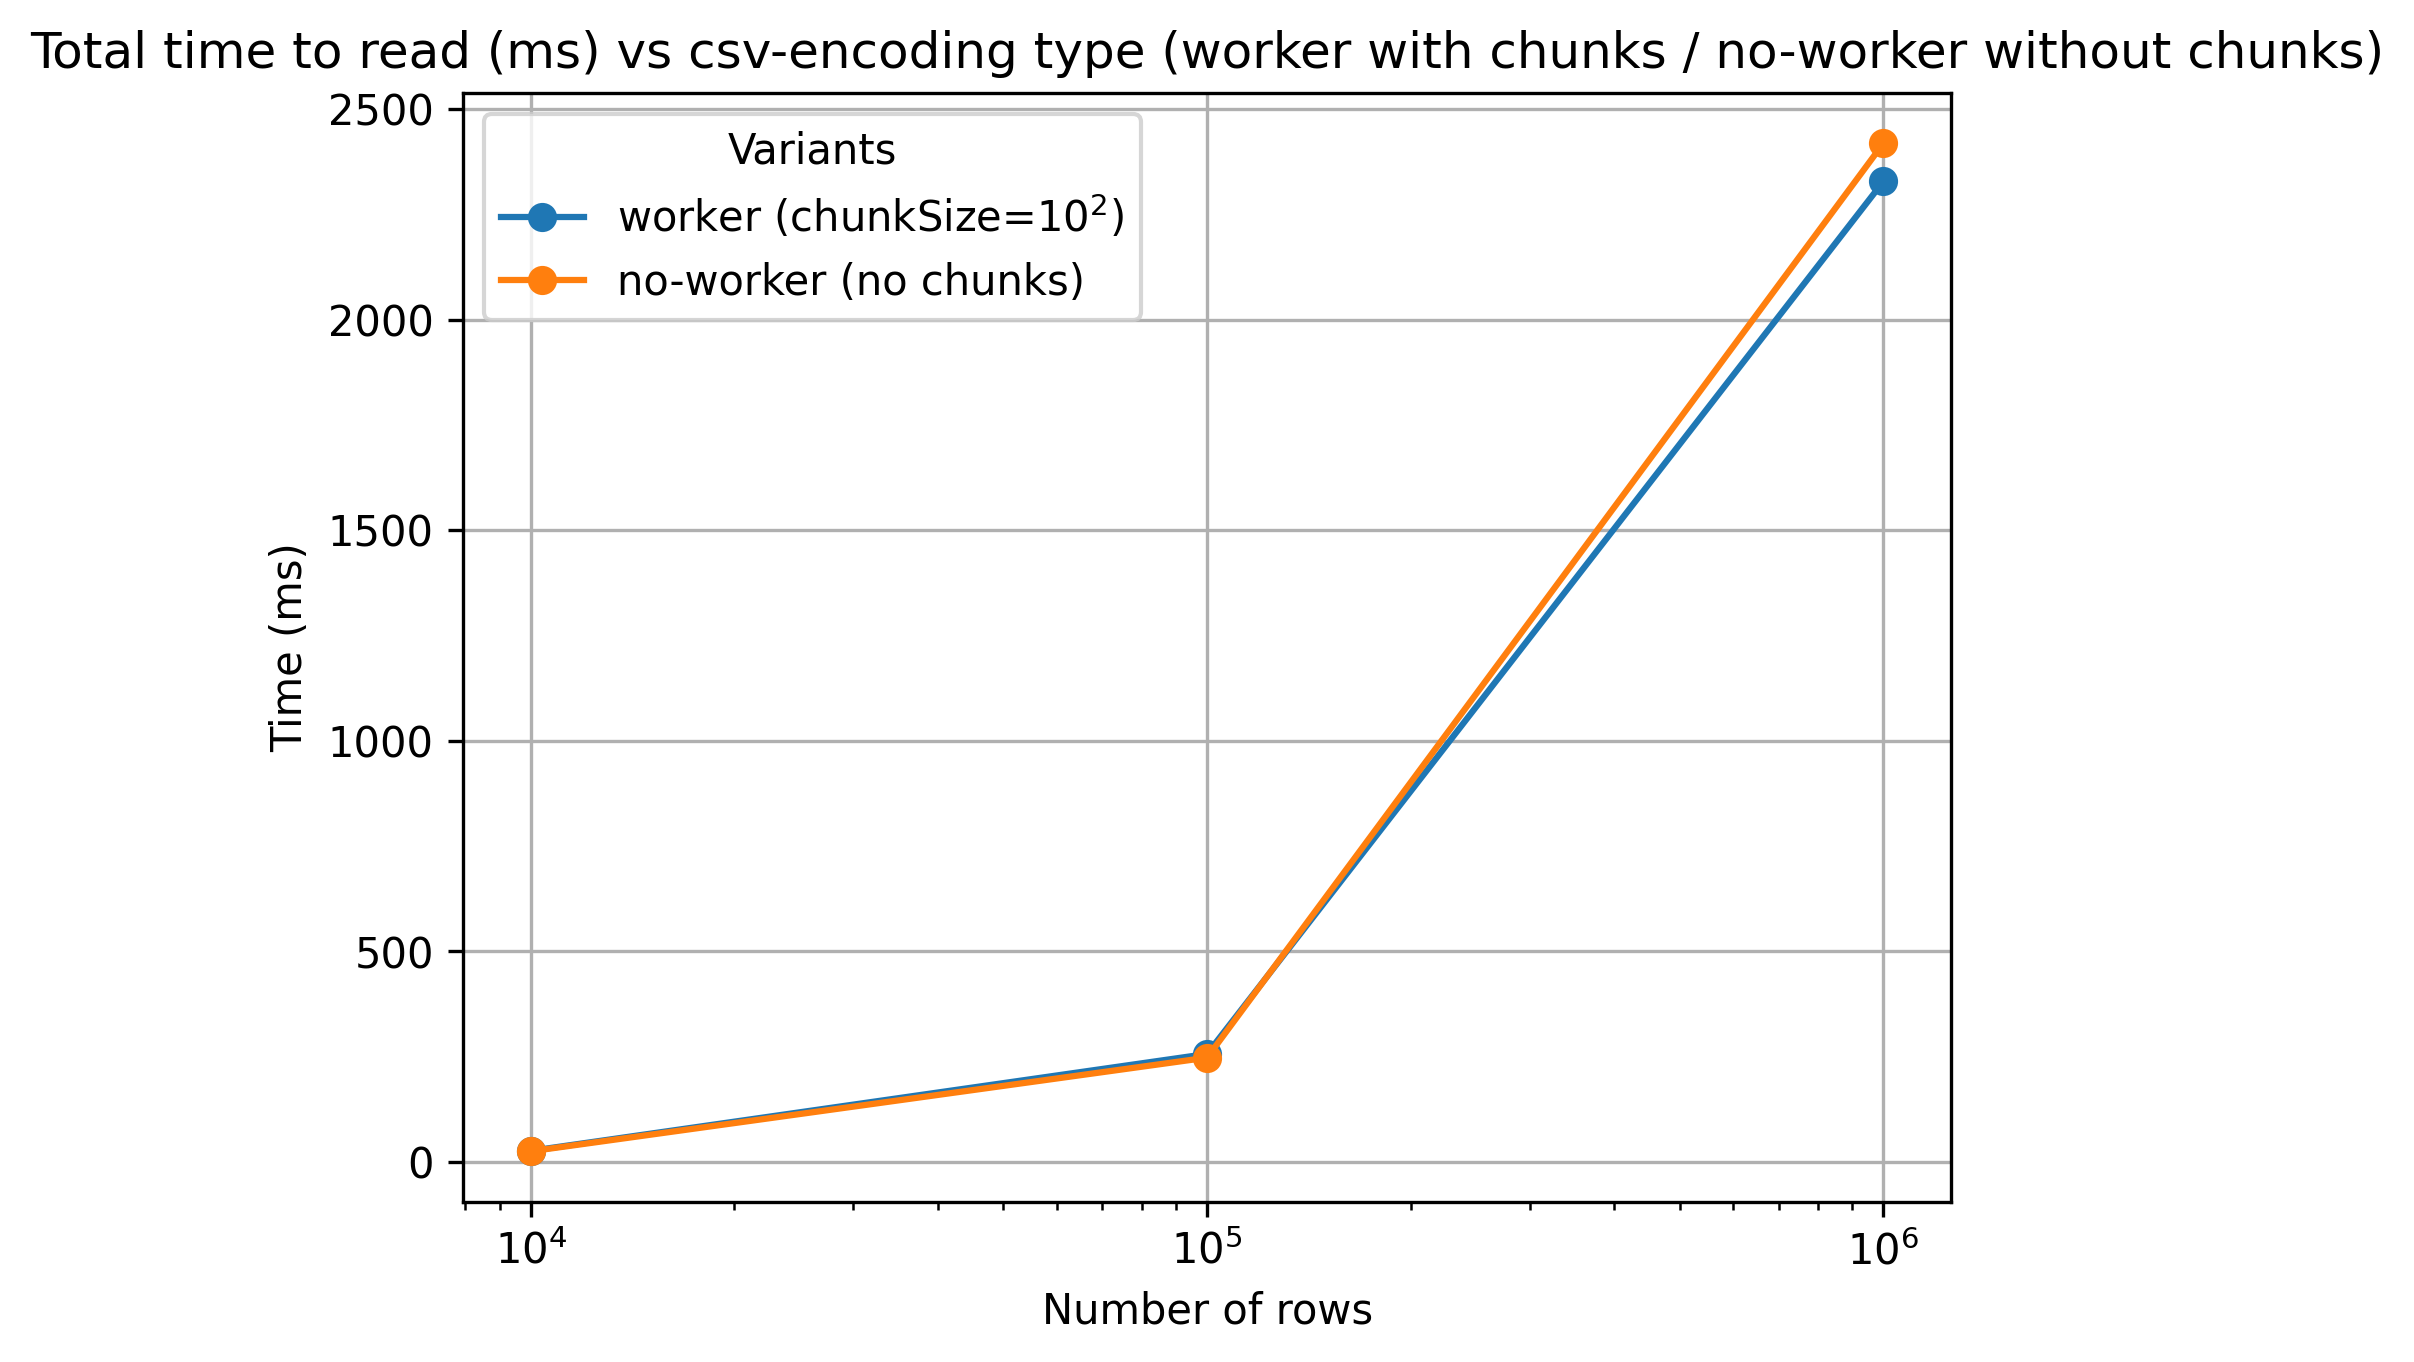
\includegraphics[scale = 0.46]{images/4-Experiments/read-input-csv-encoding.png}
    \caption*{Test for \texttt{csv} file of size up to $10^6$ rows}
  \end{minipage}
  \hfill
  \begin{minipage}{0.49\textwidth}
    \centering
    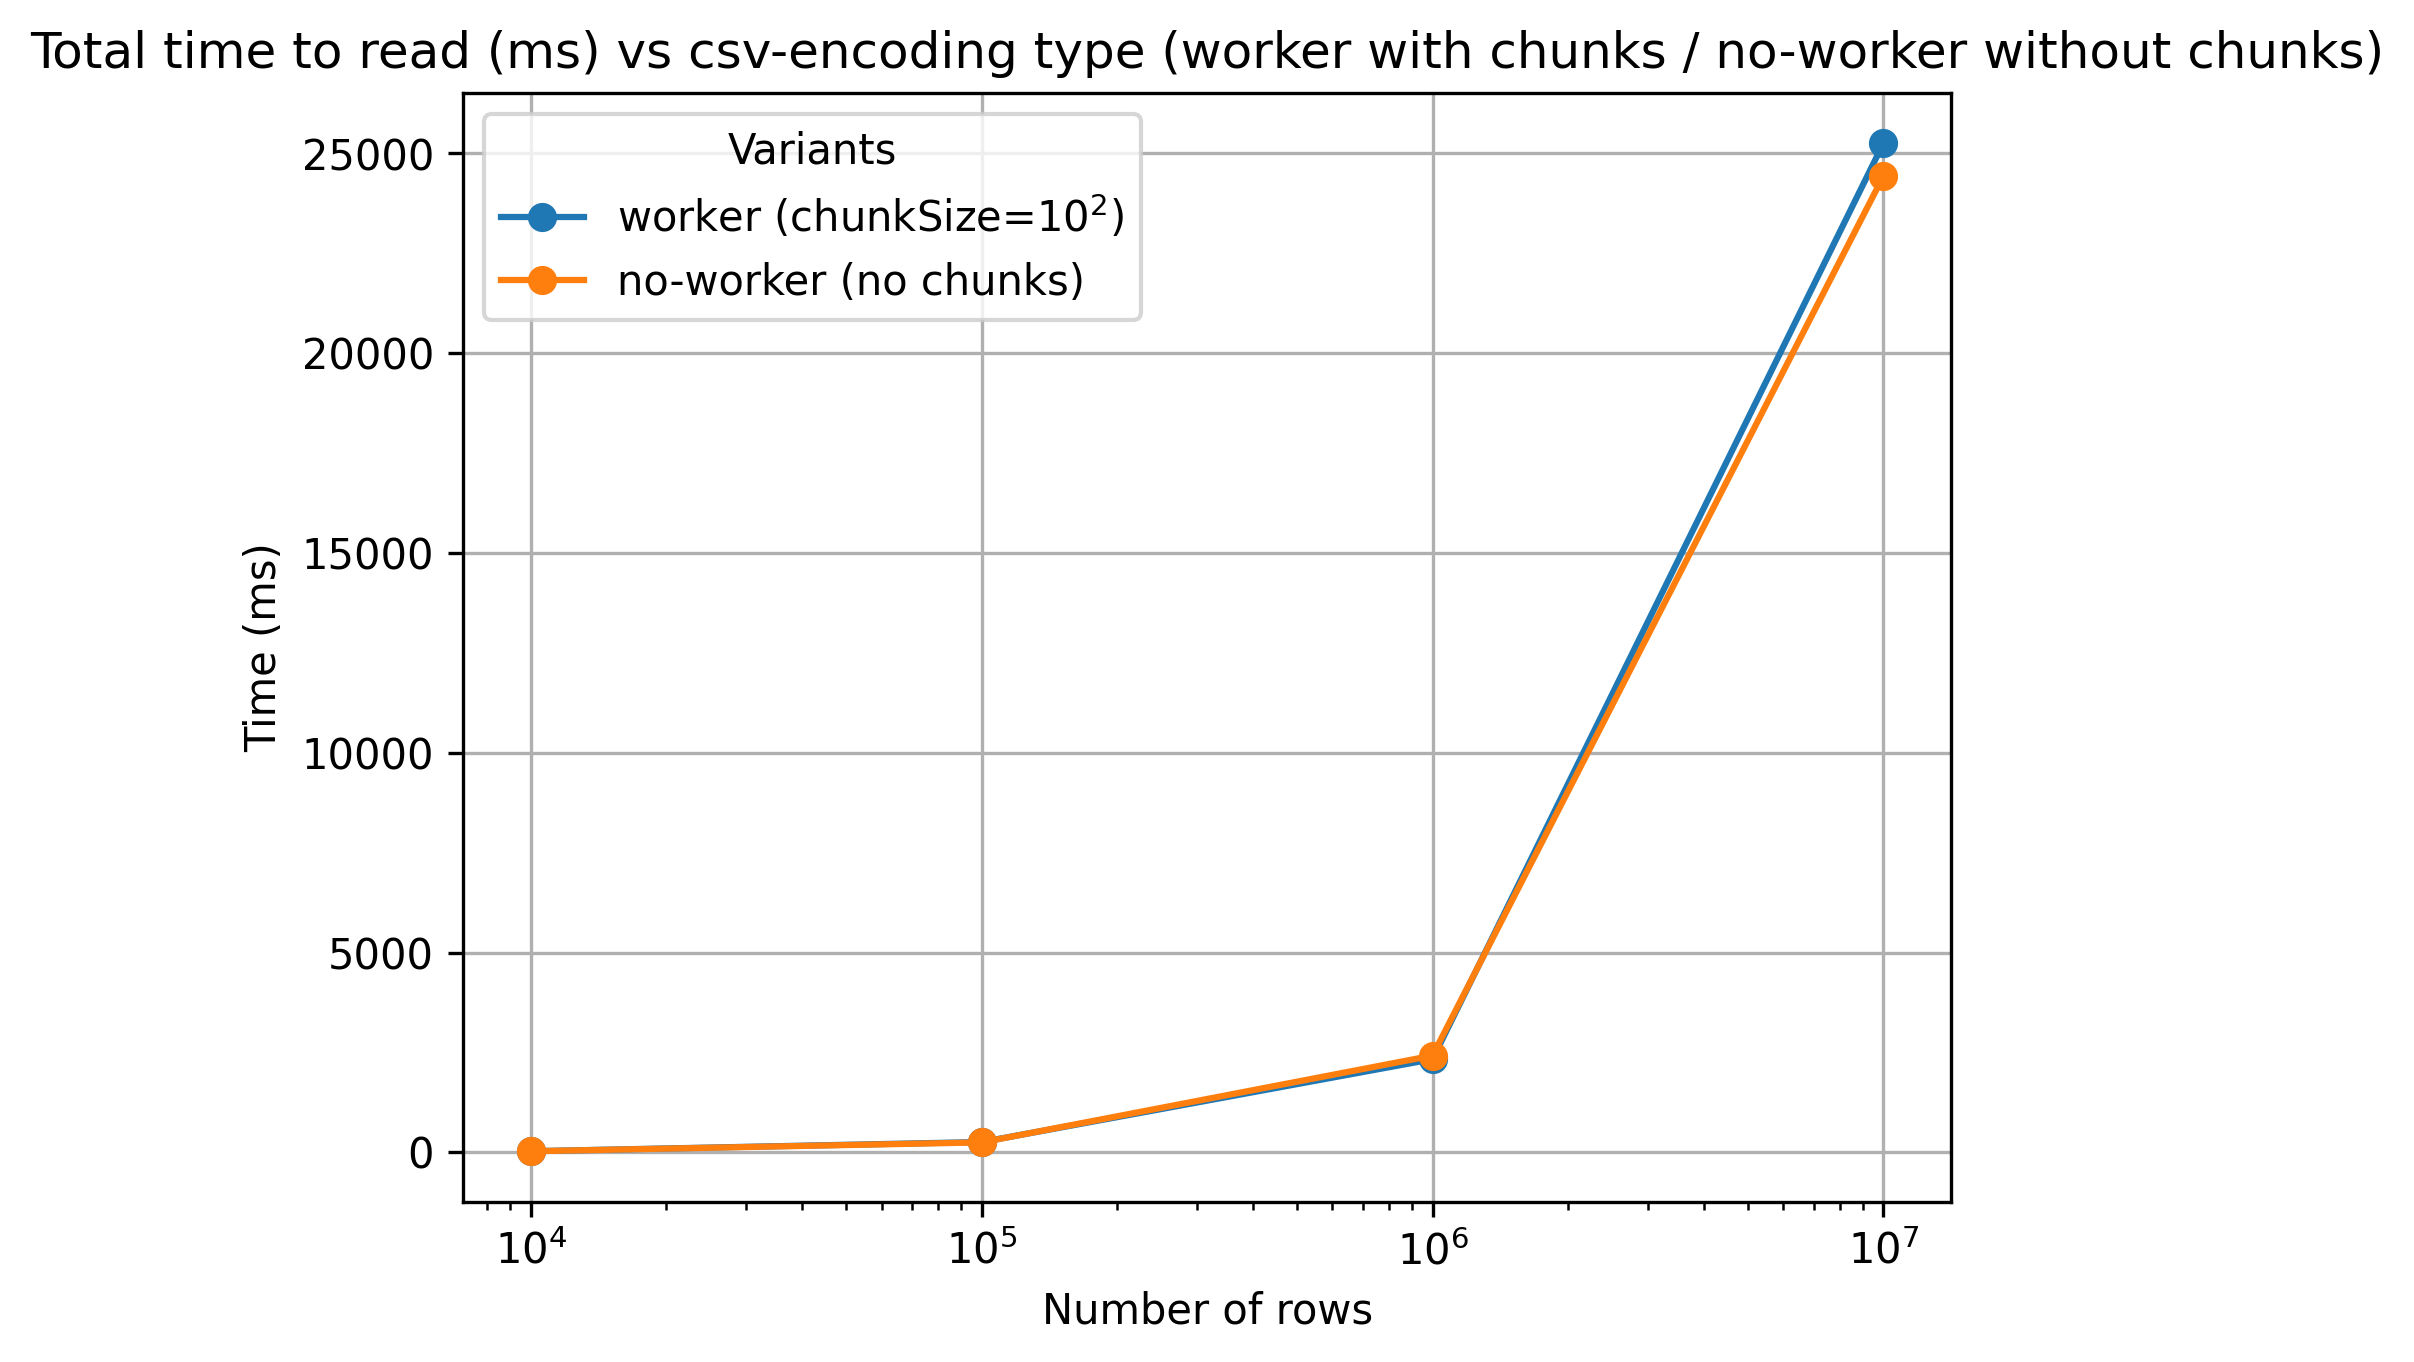
\includegraphics[scale = 0.46]{images/4-Experiments/read-input-csv-encoding-all.png}
    \caption*{Test for \texttt{csv} file of size up to $10^7$ rows}
  \end{minipage}
    \caption{Comparison of the worker and no worker variants using \texttt{encoding/csv} for reading different \texttt{csv} file sizes.}
    \label{img:exps-csv-encoding-variants}
\end{figure}

\fmc{Describir mejor el entorno}
All these experiments were run with 1 core and 1024MB of RAM at the UPC cluster.
%*******
%
